\documentclass[a4paper,12pt,oneside]{report} % définition des différents parametres. Le dernier peut-être de type report ou article (modifie le chapitrage)
	\usepackage[francais]{babel} %déclaration de la langue du document
	\usepackage[utf8]{inputenc} %déclaration du jeu de caractéres à utiliser
	\usepackage[top=2.5cm, bottom=2.5cm, left=2.5cm, right=2.5cm]{geometry} %permet de modifier les marges
	\usepackage[pdftex]{graphicx} %package nécessaire pour l'insertion d'images
	\usepackage{graphics} %package nécessaire pour l'insertion d'images 
	\usepackage{wrapfig} %package nécessaire pour l'insertion d'images
	\usepackage{amsmath} %package mathématiques (fonction \dfrac notamment)
	\usepackage{multicol} %package pour écire sur plusieurs colonnes
	\usepackage{hyperref} %package pour ajouter des liens hypertextes dans le ficher de sortie
	\usepackage{array} % meilleur gestion des tableaux
	%\usepackage{eurosym} % pour avoir notamment le symbole € --> \geneuro{}
	%\usepackage{textcomp}%pour avoir le symbole euro --> \texteuro
	\usepackage{glossaries}
	\usepackage{tikz}
	\usepackage{rotating}
	\usepackage{float}
	\usepackage{circuitikz}
	\usepackage{pdfpages}
	\usepackage{siunitx}
	\usepackage{float}
	\usepackage{xcolor}
	\usepackage{color}
	\usepackage{colortbl}
	%\usepackage[nottoc, notlof, notlot]{tocbibind}
	\usepackage[nottoc, notlot]{tocbibind}
	\usepackage{longtable}
	\usepackage{textpos}
	
	\usepackage{phdthesis}
	%\setlength{\parskip}{0.8ex}
	
	\newcolumntype{L}[1]{>{\raggedright}m{#1}}
	
		
	\title{Cours radioamateur - classe 2 \& 3} %titre du document
	\author{F4HAJ} %auteurs du document
	
	\setlongtables
	
	\makeglossaries
	\glossarystyle{long3col}	
	% pour personnaliser la façon dont sont imprimés les entrées du glossaire
	\renewcommand{\glstextformat}[1]{\textsf{#1}}
	%\renewcommand{\glstextformat}[1]{#1*}
	%\renewcommand{\glstextformat}[1]{\color{blue!70!black}\bfseries#1}
	
	%%%% debut macro %%%%
	\newenvironment{changemargin}[2]{\begin{list}{}{%
	\setlength{\topsep}{0pt}%
	\setlength{\leftmargin}{0pt}%
	\setlength{\rightmargin}{0pt}%
	\setlength{\listparindent}{\parindent}%
	\setlength{\itemindent}{\parindent}%
	\setlength{\parsep}{0pt plus 1pt}%
	\addtolength{\leftmargin}{#1}%
	\addtolength{\rightmargin}{#2}%
	}\item }{\end{list}}
	%%%% fin macro %%%%
	
	\definecolor{marron}{rgb}{0.404,0.231,0.082}
	\definecolor{orange}{rgb}{0.949,0.580,0}
	\definecolor{violet}{rgb}{0.384,0.129,0.506}
	\definecolor{gris}{rgb}{0.5,0.5,0.5}
	\definecolor{gold}{rgb}{1,0.843,0}
	\definecolor{silver}{rgb}{0.807,0.807,0.807}
	
	%page de garde
%	\makeatletter
%		\def\clap#1{\hbox to 0pt{\hss #1\hss}}%
%		\def\ligne#1{%
%		\hbox to \hsize{%
%		\vbox{\centering #1}}}%
%		\def\haut#1#2#3{%
%		\hbox to \hsize{%
%		\rlap{\vtop{\raggedright #1}}%
%		\hss
%		\clap{\vtop{\centering #2}}%
%		\hss
%		\llap{\vtop{\raggedleft #3}}}}%
%		\def\bas#1#2#3{%
%		\hbox to \hsize{%
%		\rlap{\vbox{\raggedright #1}}%
%		\hss
%		\clap{\vbox{\centering #2}}%
%		\hss
%		\llap{\vbox{\raggedleft #3}}}}%
%		\def\maketitle{%
%		\thispagestyle{empty}\vbox to \vsize{%
%		\haut{}{\@blurb}{}
%		\vfill
%		\vspace{1cm}
%		\begin{flushleft}
%		\usefont{OT1}{ptm}{m}{n}
%		\huge \@title
%		\end{flushleft}
%		\par
%		\hrule height 4pt
%		\par
%		\begin{flushright}
%		\usefont{OT1}{phv}{m}{n}
%		\Large \@author
%		\par
%		\end{flushright}
%		\vspace{1cm}
%		\vfill
%		\vfill
%		\bas{}{\@date}{}
%		}%
%		\cleardoublepage
%		}
%		\def\date#1{\def\@date{#1}}
%		\def\author#1{\def\@author{#1}}
%		\def\title#1{\def\@title{#1}}
%		\def\location#1{\def\@location{#1}}
%		\def\blurb#1{\def\@blurb{#1}}
%		\date{Avril 2012 - version 1.0}
%		\author{}
%		\title{}
%		
%		\makeatother
%		\title{Cours radioamateur - classe 2 \& 3}
%		\author{F4HAJ}
%		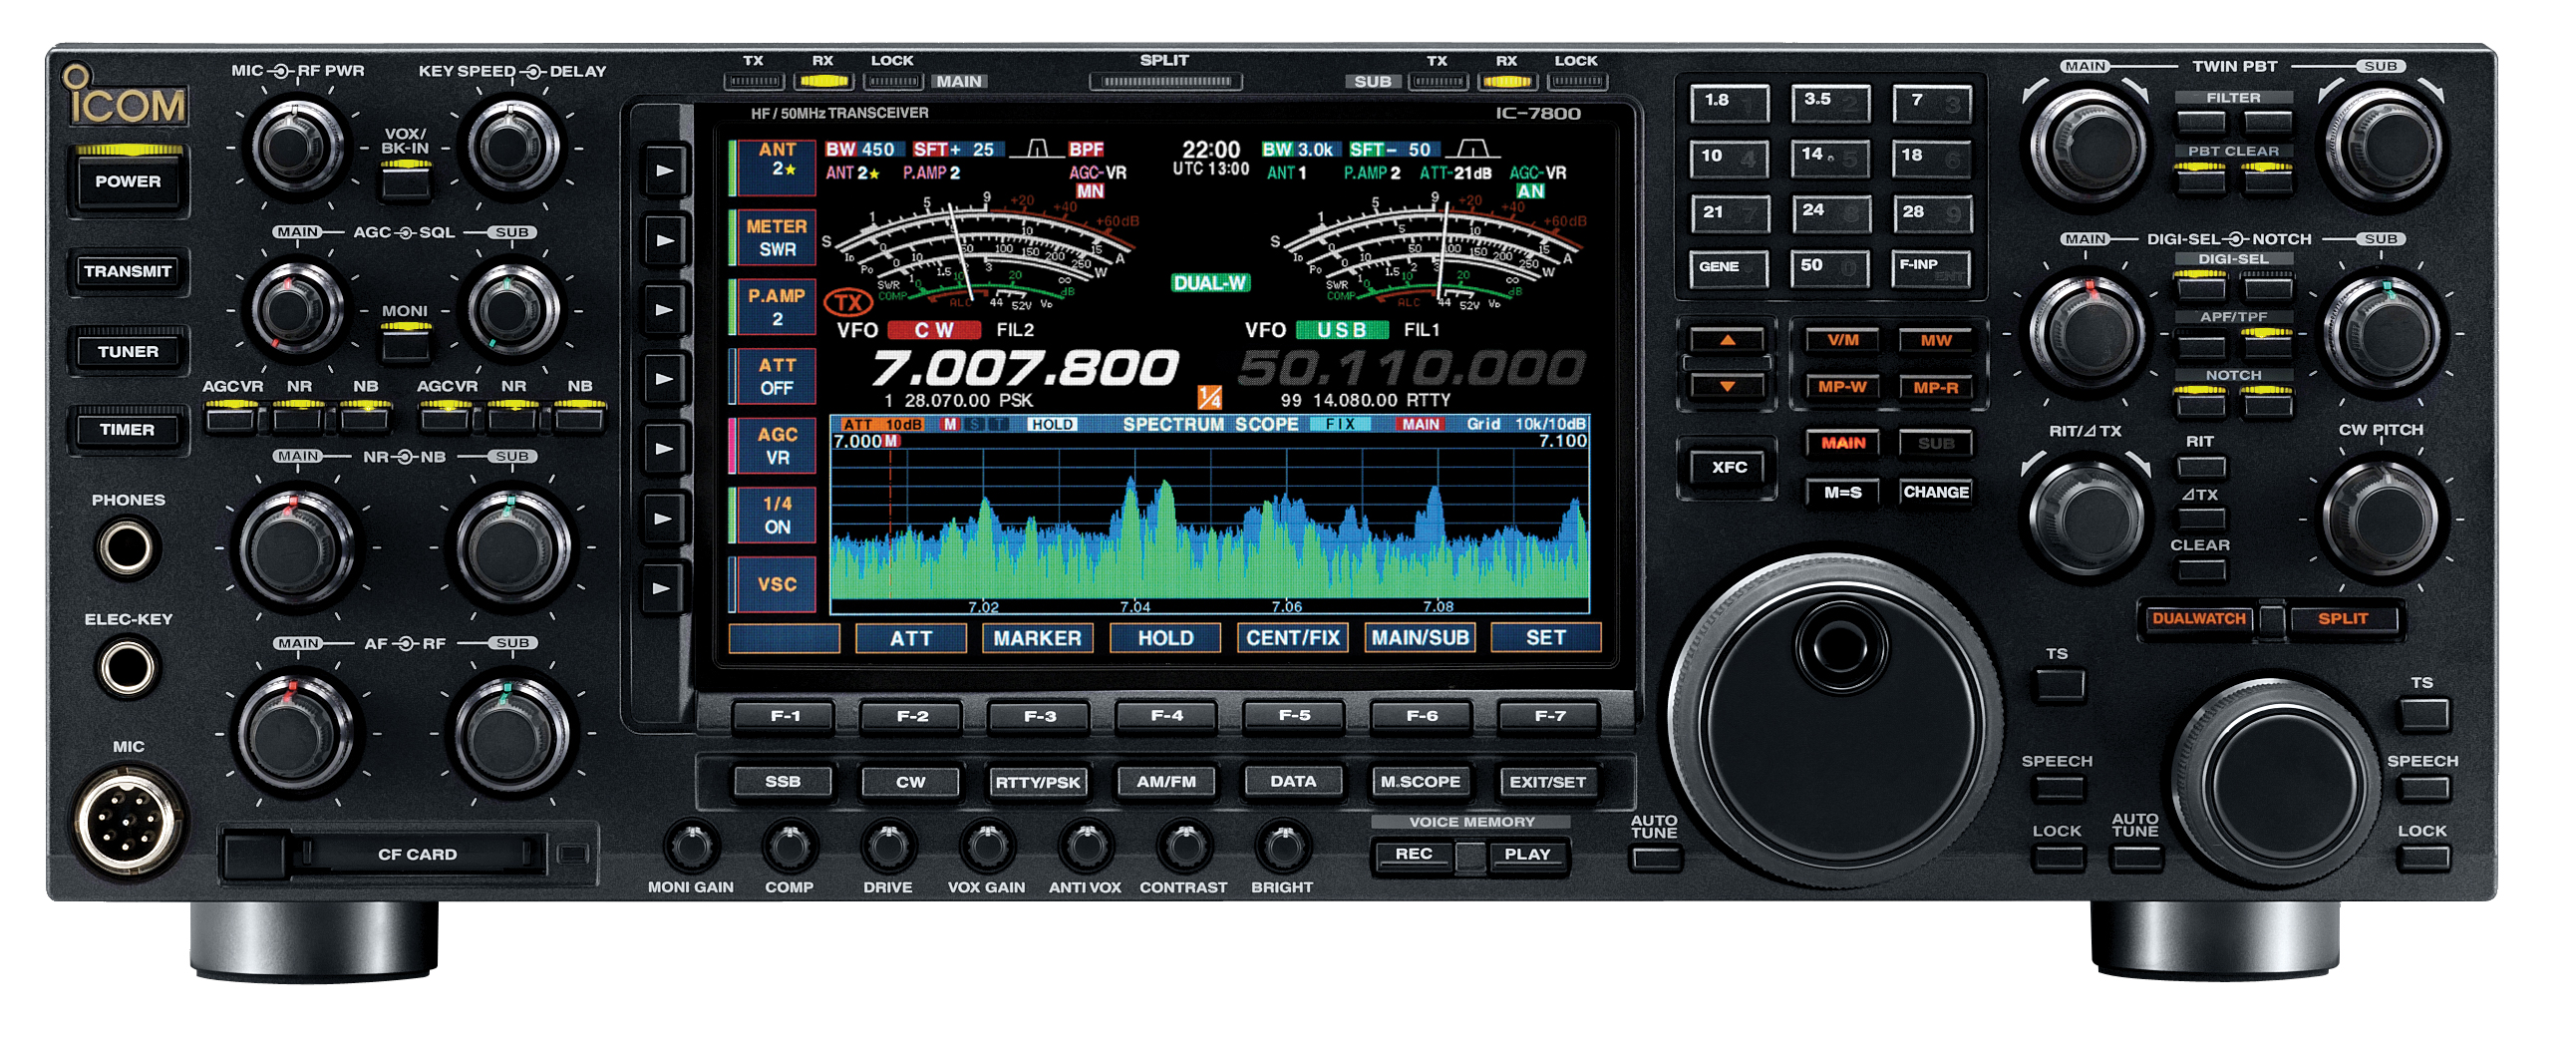
\includegraphics[scale=1]{./img/IC-7800.jpg}
%		\blurb{%
%			Test
%		}%	
	%fin page de garde
		
	
	
	
	
	
	\begin{document}
	
	\begin{titlepage}%ta page de titre 
		\begin{center} 
			~
			\vfill
			\begin{flushleft}
				\usefont{OT1}{ptm}{m}{n}
				\huge Cours radioamateur - classe 2 \& 3
			\end{flushleft}
			\par
			\hrule height 4pt
			\par
			\begin{flushright}
				\usefont{OT1}{phv}{m}{n}
				\Large F4HAJ
				\par
			\end{flushright}
			\vspace{2cm}
			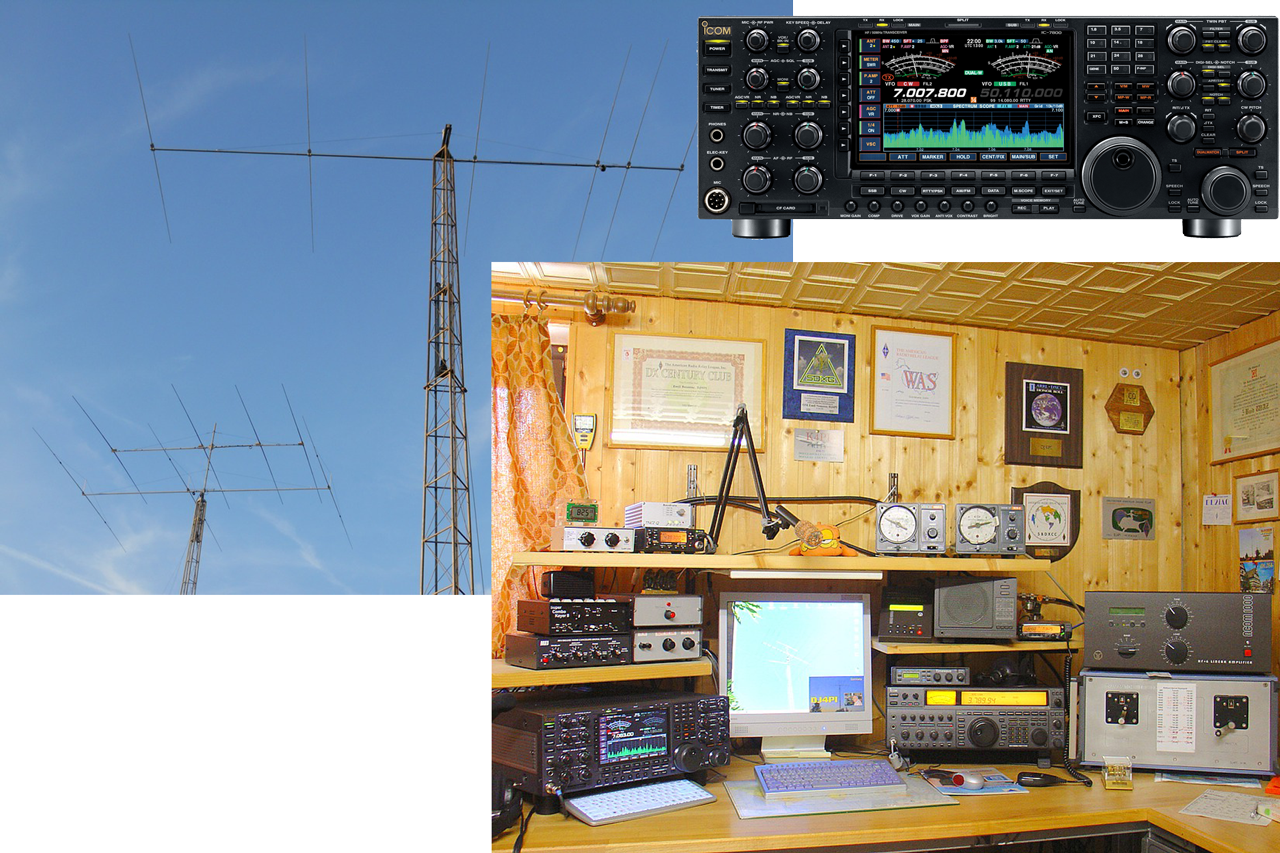
\includegraphics[width=\textwidth]{./img/img_couverture.png} 
			\vfill
			\vfill
		\end{center}
			\begin{textblock*}{30mm}[0,0](-20mm,-25mm)
				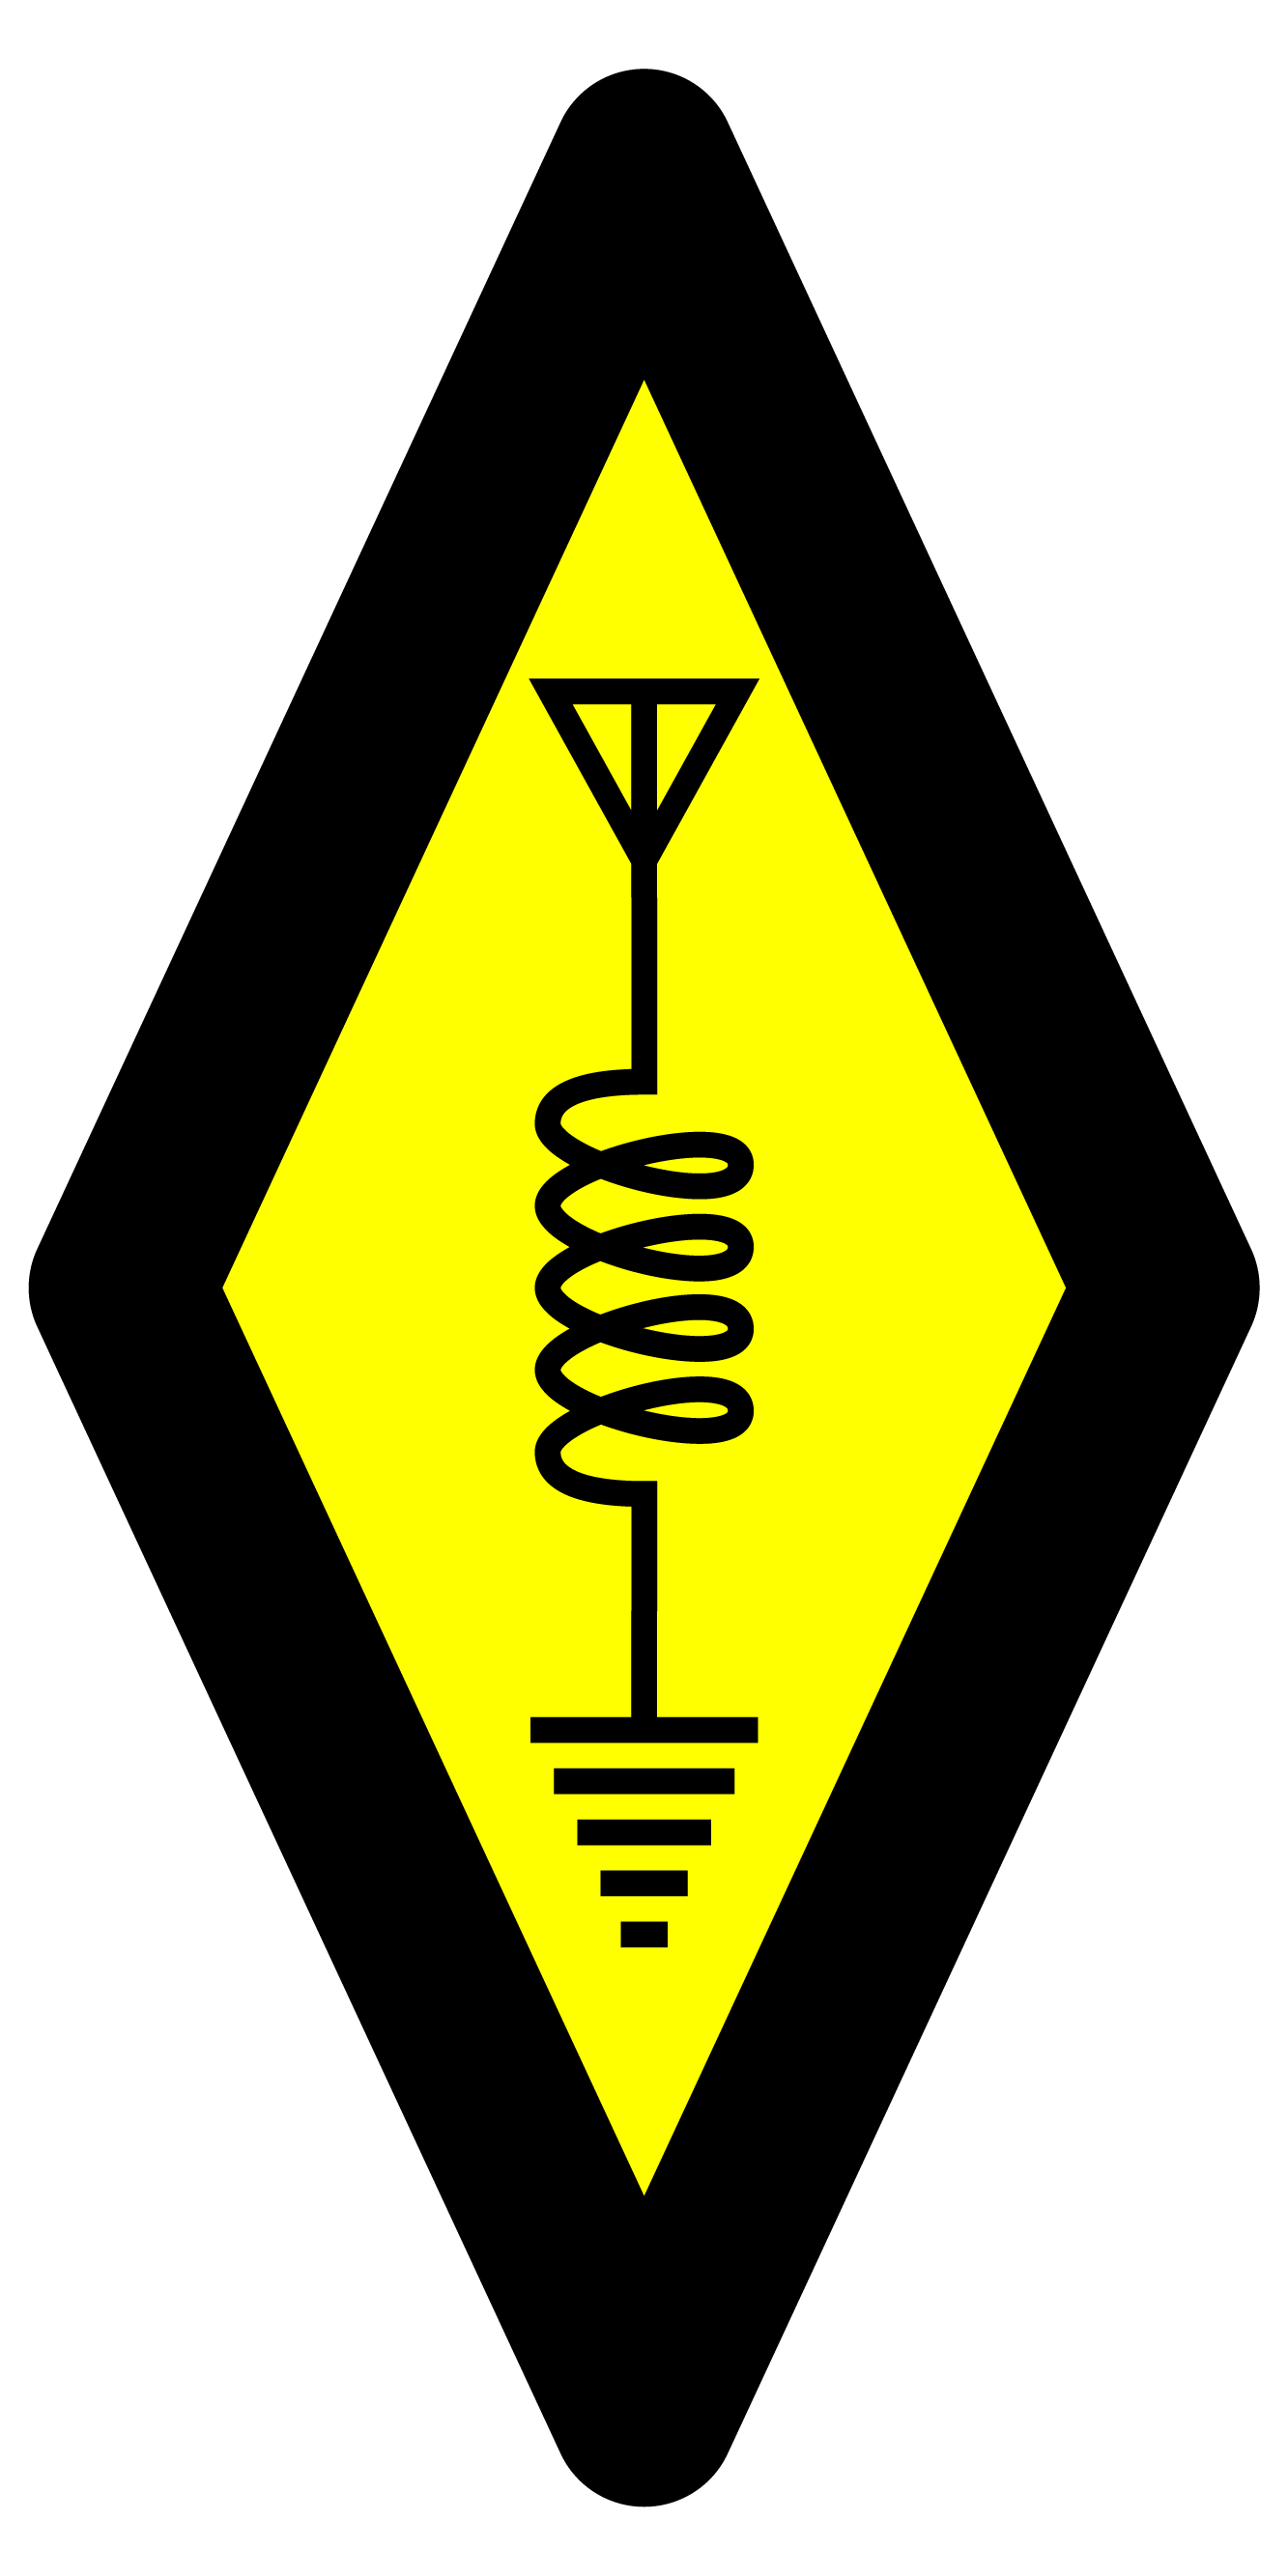
\includegraphics[width=3cm]{./img/International_symbol.png} 
			\end{textblock*}
		\begin{center}
			http://f4haj.net
			
			Août 2012 - version 1.1
		\end{center} 
	\end{titlepage} 	
	

	\tableofcontents
	\newpage	
	
	\section{Préface}
	%\alert{test}
	%\info{test}
	%\question{test}

	Ce document était à la base un simple memento destiné à mon usage propre en vue du passage des licences classe 2 et 3 d'opérateur du service amateur. Il est devenu, au fur et à mesure de mon apprentissage, un document résumant de façon synthétique (je pense), les principales notions nécessaires à la préparation de ces licences. Ce document m'a permis de préparer et de passer simultanément et avec succès les examens de législation et de technique, et ceci en seulement 2 mois de préparation.

	J'ai décidé de le diffuser car je trouve qu'il n'est pas facile de trouver sur Internet des cours à la fois complets et synthétiques pour la préparation de la licence radioamateur française.

	Je ne prétend pas que l'approche adoptée dans ce document conviendra à tout le monde. Ce document regroupe les principales notions et formules à connaitre. Il peut servir de base pour la préparation d'une licence ou encore de memento pour le maintient des connaissances après l'obtention de la licence. Je continue de penser que l'adhésion à un radioclub demeure indispensable, ne serais-ce que pour donner un certaines synergie à cet apprentissage passionnant mais qui peut parfois paraître fastidieux. Par ailleurs, les informations et conseils que pourront vous fournir les membres d'un radioclub seront toujours utiles et bienvenus, y compris après l'obtention de la licence (conseil sur le matériel, le montage d'une antenne...).

	Enfin, ce document est destiné à évoluer. Je souhaite ajouter de nouvelles notions prochainement pour ceux qui souhaiteraient aller plus loin. Par ailleurs, je suis ouvert à toutes critiques ou commentaires constructifs concernant ce document, sur le fond comme sur la forme. N'hésitez donc pas à me contacter concernant toute erreur, omission, faute d'orthographe ou manque dans ce documents, à l'adresse contact@f4haj.net.

	\section{Licence}
	Ce document est diffusé sous licence Creative Commons 3.0 by-nc-sa dont les termes sont disponibles sur le site CreativeCommons.org\footnote{Termes disponibles à cette adresse : \url{http://creativecommons.org/licenses/by-nc-sa/3.0/}}. De façon synthétique, cette licence \textbf{vous autorise à redistribuer et à modifier ce document tant que vous le souhaitez tant que vous me citez en tant qu'auteur original} (un lien vers la version vous ayant servit de base est souhaité). En cas de diffusion de la version modifiée, vous avez l'obligation de la diffuser sous la même licence. Toute utilisation commerciale est en revanche proscrite. Si vous souhaitez \textbf{faire un usage dépassant le cadre de cette licence} (donc utilisation commerciale, diffusion sous une autre licence...),vous devez \textbf{impérativement obtenir mon autorisation expresse écrite}. Pour cela vous pouvez me contacter à l'adresse contact@f4haj. Je tiens par ailleurs à votre disposition le fichier source \LaTeX{} de ce document sur simple demande.

	\chapter{Quelques rappels}
		\section{Multiples et sous-multiples}
			Nous verront plus loin que dans de nombreux cas, on est amené à manipuler des chiffres importants (de l'ordre du million par exemple) ou au contraire très petits (de l'ordre du millième de milliardième). Par exemple, une résistance pourrait avoir une valeur de $1000000 \Omega$ (un million d'ohms). Ou encore, un condensateur (nous verront ce que c'est plus loin), une capacité de $0,000 000 000 001 F$ (un millionième de milliardième de Farad). Ces valeurs, avec un grand nombre de 0, ne sont ni simples à lire, ni très pratiques, car on peut facilement oublier ou ajouter un 0, ce qui changera le résultat final. Pour éviter ce problème, on à inventé des multiples et des sous multiples. Vous en utilisez déjà dans la vie des tous les jours, avec les distances par exemple. Tout le monde connait les mètres, auxquels on à ajouté le kilomètre ($1000 m$) et le millimètre (1 millième de mètre soit $0,001 m$). Entre le milli et le kilo, on trouve le centimètre ($0,01 m$), le décimètre ($0,1 m$), le mètre ($1 m$), le décamètre ($10 m$) et enfin l'hectomètre ($100 m$). Ces unités, on les utilises tous les jours, et il y a fort a parier que vous savez pas sans trop de problèmes de l'une à l'autre.
    
    Comme ces unités "usuelles" ne sont pas encore assez grandes (ou assez petites) pour nos besoins, on en a inventé d'autres. Commençons par les multiples :
    
    \begin{center}
        \begin{tabular}{|c|c|c|c|c|c|c|c|c|c|c|}
        \hline
            & \multicolumn{3}{c|}{Giga} & \multicolumn{3}{c|}{Méga} & Kilo & Hecto & Deca & unité \\
            Symbole & \multicolumn{3}{c|}{G} & \multicolumn{3}{c|}{M} & K & h & da & \\
        \hline
    	    Nombre de 0 à ajouter & \multicolumn{3}{c|}{9} & \multicolumn{3}{c|}{6} & 3 & 2 & 1 & 0 \\
            
        \hline
        \end{tabular}
    \end{center}
	Les sous mutliples : 
    \begin{center}
        \begin{tabular}{|c|c|c|c|c|c|c|c|c|c|c|c|c|c|}
            \hline
                & unité & deci & centi & milli & \multicolumn{3}{c|}{micro} & \multicolumn{3}{c|}{nano} & \multicolumn{3}{c|}{pico}\\
                Symbole & & d & c & m & \multicolumn{3}{c|}{$\mu$} & \multicolumn{3}{c|}{n} & \multicolumn{3}{c|}{p}  \\
        	\hline
        	    Nombre de 0 à ajouter & 0 & 1 & 2 & 3 & \multicolumn{3}{c|}{6} & \multicolumn{3}{c|}{9} & \multicolumn{3}{c|}{12} \\      
            \hline
        \end{tabular}
    \end{center}

	Enfin, le tableau entier :
    \begin{center}
        \begin{tabular}{|c|c|c|c|c|c|c|c|c|c|c|c|c|c|c|c|c|c|c|c|c|c|c|c|c|c|}
            \hline
                \multicolumn{3}{|c|}{Giga} & \multicolumn{3}{c|}{Méga} & Kilo & Hecto & Deca & unité & deci & centi & milli & \multicolumn{3}{c|}{micro} & \multicolumn{3}{c|}{nano} & \multicolumn{3}{c|}{pico}\\
                \multicolumn{3}{|c|}{G} & \multicolumn{3}{c|}{M} & K & h & da & & d & c & m & \multicolumn{3}{c|}{$\mu$} & \multicolumn{3}{c|}{n} & \multicolumn{3}{c|}{p}  \\
        	\hline
        \end{tabular}
    \end{center}

	Ainsi, vous entendrez parfois un radioamateur qu'il a fait du "décamétrique". Cela signifie donc qu'il a trafiqué dans les bandes dont les unités se comptent en dizaines de mètres. La longueur d'onde utilisée va donc de 10 m à 100 m (donc de 1 à 10 dam).

	Il faut faire très attention aux unités, car il n'est pas possible d'additionner deux grandeurs qui ne se trouvent pas dans les mêmes unités. Par exemple, on vous demande de donner la valeur de la somme de deux résistance. La première fait $7,6 M\Omega$ (7,6 mégaohm) et la deuxième fait $15 k\Omega$ (15 kiloohm). Un candidat distrait fera la somme $7,6 + 15 = 21,6$ et répondra faux. Pour additionner, il faut remettre toutes les valeurs dans les mêmes unités. C'est très simple avec un tableau :

\begin{center}
    \begin{tabular}{|c|c|c|c|c|c|c|c|c|c|c|c|c|c|c|c|c|c|c|c|c|c|c|c|}
        \hline
              \multicolumn{3}{|c|}{\begin{sideways}Giga\end{sideways}} & \multicolumn{3}{c|}{\begin{sideways}Méga\end{sideways}} & \multicolumn{3}{c|}{\begin{sideways}Kilo\end{sideways}} & \begin{sideways}Hecto\end{sideways} & \begin{sideways}Deca\end{sideways} & \begin{sideways}unité\end{sideways} & \begin{sideways}deci\end{sideways} & \begin{sideways}centi\end{sideways} & \begin{sideways}milli\end{sideways} & \multicolumn{3}{c|}{\begin{sideways}micro\end{sideways}} & \multicolumn{3}{c|}{\begin{sideways}nano\end{sideways}} & \multicolumn{3}{c|}{\begin{sideways}pico\end{sideways}} \\
           \multicolumn{3}{|c|}{G} & \multicolumn{3}{c|}{M} & \multicolumn{3}{c|}{K} & h & da & & d & c & m & \multicolumn{3}{c|}{$\mu$} & \multicolumn{3}{c|}{n} & \multicolumn{3}{c|}{p}  \\
    	\hline
    		&&&&&7& 6  &0&0&0&0&0&&&&&&&&&&&& \\
			&&&&&&&1&5&0&0&0&&&&&&&&&&&& \\
		\hline
			&&&&&7&6&1&5&0&0&0&&&&&&&&&&&& \\
		\hline
    \end{tabular}
\end{center}


		\section{Electricité - montage parallèle et série}
			\subsection{Tension et intensité}
				Il existe 2 valeurs fondamentales lorsque l'on parle d'électricité : la tension et l'intensité. Ces 2 notions sont très importantes à connaitre car elles servent de base pour l'ensemble des autres mesures que l'on peut faire sur un circuit électrique ! Il est également nécessaire de savoir comment mesurer ces valeurs.
				\subsubsection{La tension}
				La tension existe parce qu'il existe une \textbf{différence de potentiel} entre les bornes d'un générateur. Mais qu'es-ce que la différence de potentiel ? Prenons un chute d'eau (une cascade par exemple). La différence de hauteur entre le point haut de la chute et le point bas représente la différence de potentiel.

				La tension se mesure en volts (symbole V), à l'aide d'un \textbf{voltmètre}. Un voltmètre se \textbf{se place toujours en dérivation} dans un circuit.

				Propriétés d'un voltmètre
				\begin{itemize}
					\item Résistance très élevée (un voltmètre parfait aurait une résistance infinie)
					\item Se place en parallèle dans le circuit
				\end{itemize}

				\subsubsection{L'intensitée}
			\subsection{Montage parallèle}
			Le montage d'un circuit en parallèle (on parle également de montage en dérivation) est le montage le plus répandu, et pour cause, c'est ce montage qui est utilisé dans les circuits électriques de nos habitations. Dans ce montage, tous les 2 bornes du consommateurs sont reliées directement aux 2 bornes du générateur.

	\begin{center}
	    \shorthandoff{:!}
		\begin{circuitikz}[european] \draw
			(0,0) to [lamp, l_=$L_1$] (0,2)
			(2,0) to [lamp, l_=$L_2$] (2,2)
			(4,0) to [lamp, l_=$L_3$] (4,2)
			(-2,0) to [battery] (-2,2)
			(-1,0) to[short] (-2,0) %node[anchor=east]{A}
			(-1,2) to[short] (-2,2) %node[anchor=east]{B}
			(-1,0) -- (4,0)
			(-1,2) -- (4,2)
		;\end{circuitikz}
		\shorthandoff{:!}
	\end{center}

			Les propriétés d'un circuit parallèle sont les suivantes :
			\begin{itemize}
				\item La tension est la même aux bornes de tous les consommateurs
				\item L'intensité débitée par le générateur est égale à la somme des intensités des consommateurs
				\item Si un consommateur est débranché ou cesse de fonctionner, les autres consommateurs continuent de fonctionne normalement	
			\end{itemize}

			\subsection{Montage en série}
			On parle de montage en série lorsque les éléments d'un circuit sont branchées les uns à la suite des autres.

\begin{center}
        \shorthandoff{:!}
		\begin{circuitikz}[european] \draw
			(0,0) to [lamp, l_=$L_1$] (2,0)
			(2,0) to [lamp, l_=$L_2$] (4,0)
			(4,0) to [lamp, l_=$L_3$] (6,0)
			(2,2) to [battery] (4,2)
			(2,2) to[short] (-0.5,2)
			(4,2) to[short] (6.5,2)
			(6.5,0) to[short] (6.5,2)
			(-0.5,2) to[short] (-0.5,0) 
			(0,0) to[short] (-0.5,0) 
			(6,0) to[short] (6.5,0)
		;\end{circuitikz}
		\shorthandoff{:!}
	\end{center}
			

			Les propriétés d'un circuit série sont les suivantes :
			\begin{itemize}
				\item La tension aux bornes du générateur est égale à la somme des tensions mesurée aux bornes de chaque consommateur
				\item L'intensité du courant dans un circuit série est la même en tout points du circuit
				\item Le débranchement ou la panne de l'un des consommateurs provoque l'arrêt des autres consommateurs (le circuit n'est plus fermé)
			\end{itemize}
   
	
	\chapter{Réglementation}
		\section{Tableau des fréquences - région 1}
		Voici un tableau présentant les bandes de fréquences les plus souvent demandées à l'examen. Un tableau complet est disponible en annexe, section \ref{frequencyAllocationFull}, page \pageref{frequencyAllocationFull}.
		\begin{center}
		\begin{longtable}{|L{2.0cm}|L{2.0cm}|L{6.23cm}|L{1.1cm}|L{1.3cm}|L{0.5cm}|}
			\hline
			\multicolumn{2}{|c|}{Bande} & & & &\tabularnewline
			
			Limite basse & Limite haute & Statut & Longu- -eur & Largeur de la bande & Sat \tabularnewline
			\hline
			135,7~kHz 	& 137,8~kHz & \cellcolor{red} bande partagée statut secondaire & 2222~m & 2,1~kHz &  \tabularnewline
			\hline
			1,810~MHz & 1,850~MHz & \cellcolor{green} bande exclusive & 160 m &40~kHz & \tabularnewline
			\hline
			3,500~MHz & 3,800~MHz & \cellcolor{yellow} bande partagée à égalité de droit & 80 m & 300~kHz & \tabularnewline
			\hline
			7,000~MHz & 7,200~MHz & \cellcolor{green} bande exclusive & 40 m & 200~kHz & $\uparrow \downarrow$\tabularnewline
			\hline
			10,100~MHz & 10,150~MHz & \cellcolor{red} bande partagée statut secondaire & 30 m & 50~kHz & \tabularnewline
			\hline
			14,000~MHz & 14,350~MHz & \cellcolor{green} bande exclusive & 20 m & 350~kHz & $\uparrow \downarrow$\tabularnewline
			\hline 
			18,068~MHz & 18,168~MHz & \cellcolor{green} bande exclusive & 17 m & 100~kHz & $\uparrow \downarrow$\tabularnewline
			\hline
			21,000~MHz & 21,450~MHz & \cellcolor{green} bande exclusive & 15 m & 450~kHz & $\uparrow \downarrow$\tabularnewline
			\hline
			24,890~MHz & 24,990~MHz & \cellcolor{green} bande exclusive & 12 m & 100~kHz & $\uparrow \downarrow$\tabularnewline
			\hline
			28,000~MHz & 29,700~MHz & \cellcolor{green} bande exclusive & 10 m & 1,7~MHz & $\uparrow \downarrow$\tabularnewline
			\hline
			50,200~MHz & 51,200~MHz &\cellcolor{black}  \textcolor{white}{bande partagée statut dérogatoire} & 6 m & 1~MHz & \tabularnewline
			\hline
			144,00~MHz & 146,00~MHz & \cellcolor{green} bande exclusive & 2 m & 2~MHz & $\uparrow \downarrow$\tabularnewline
			\hline
			430,00~MHz & 434,00~MHz & \cellcolor{red} bande partagée statut secondaire & 70 cm & 4~MHz & \tabularnewline
			\hline
			434,00~MHz & 440,00~MHz & \cellcolor{yellow} bande partagée à égalité de droit & 70 cm & 6~MHz & $\uparrow~*$  \tabularnewline
			\hline
			1240,0~MHz & 1300,0~MHz & \cellcolor{red} bande partagée statut secondaire & 23 cm & 60~MHz & $\uparrow $ \tabularnewline
			\hline
		\end{longtable}
		\end{center}
		
		\subsection{Mnémotechnique sur les bandes}
		\begin{enumerate}
			\item Bandes à statut exclusif : 1,8 MHz + multiples de 6 + multiples de 7
			\item Bande partagée à statut secondaire : 135.7 kHz + bandes dont la limite basse est multiple de 10 (sauf 50 MHz dérogatoire)
			\item Toutes les autres bandes sont à égalité de droits
		\end{enumerate}
		
		\section{Spectre et dénomination}
			\begin{center}
			\begin{longtable}{|L{2cm}|L{3.5cm}|L{3.5cm}|L{4.5cm}|}
				\hline
				Désignation & Fréquence & Longueur d'onde & Appellation \tabularnewline
				\hline
				VLF & 3 kHz à 30 kHz & 100 km à 10 km & Ondes myriamétriques \tabularnewline
				\hline
				LF & 30 kHz à 300 kHz & 10 km à 1 km & Ondes kilométriques \tabularnewline
				\hline
				MF & 300 kHz à 3 MHz & 1 km à 100 m & Ondes hectométriques \tabularnewline
				\hline
				HF & 3 MHz à 30 MHz & 100 m à 10 m & Ondes décamétriques \tabularnewline
				\hline
				VHF & 30 MHz à 300 MHz & 10 m à 1 m & Ondes métriques \tabularnewline
				\hline
				UHF & 300 MHz à 3 GHz & 1 m à 10 cm & Ondes décimétriques \tabularnewline
				\hline
				SHF & 3 GHz à 30 GHz & 10 cm à 1 cm & Ondes centimétrique \tabularnewline
				\hline
				EHF & 30 GHz à 300 GHz & 1 cm à 1 mm & Ondes millimétriques \tabularnewline
				\hline
			
			\end{longtable}
			\end{center}
			
		\section{Classes d'émissions}
		Les classes d'émissions est un système codifié, mis en place et reconnu par l'UIT et qui permet d'identifier les classes d'émissions.

		Voici les principales classes utiles en France (classes à connaitre pour l'examen). Il existe d'autres classes d'émissions, le tableau complet est disponible en section \ref{emittingClassesFull}, page \pageref{emittingClassesFull}.
		\begin{center}
	  	\begin{longtable}{|L{1.5cm}|L{7cm}|L{5cm}|}
	      \hline
	      Symbole & Signification & Mnémotechnique \tabularnewline
	    	\hline
			\hline
	      \textbf{A} & Modulation d'\textbf{a}mplitude, double bande latérale, porteuse normale & \textbf{A} comme \textbf{a}mplitude  \tabularnewline
	      \hline
			\textbf{R} & Modulation d'amplitude, bande latérale unique, porteuse \textbf{r}éduite & \textbf{R} comme \textbf{r}éduite  \tabularnewline
	      \hline
	\textbf{J} & Modulation d'amplitude,  bande latérale unique, porteuse supprimée & \textbf{J} comme \textbf{j}amais de sous porteuse  \tabularnewline
	      \hline
		\textbf{C} & Modulation d'amplitude, bande latérale résiduelle & \textbf{C} comme \textbf{C}résiduelle (résiduelle)  \tabularnewline
		\hline
		\textbf{F} & Modulation de \textbf{f}réquence & \textbf{F} comme \textbf{F}réquence  \tabularnewline
		\hline
		\textbf{G} & Modulation de phase & on utilise une antenne en hélice, comme un \textbf {G}  \tabularnewline
	     	\hline
			\hline
		\textbf{1} & Signal digital sans emploi d'un sous porteuse modulance & Le \textbf{1} est \textbf{sans emploi}  \tabularnewline
	      \hline
		\textbf{2} & Signal digital avec  emploi d'une sous porteuse modulante & Le \textbf{2} est \textbf{avec emploi}  \tabularnewline
		\hline
		\textbf{3} & Signal analogique (voix, image...) &  \tabularnewline
		\hline
		\textbf{7} & Plusieurs voix contenant de l'information numérique &  \tabularnewline
		\hline
		\hline
		\textbf{A} & Télégraphie pour réception auditive & \textbf{A} comme \textbf{auditive}  \tabularnewline
		\hline
		\textbf{B} & Télégraphie pour réception automatique & \textbf{B} comme \textbf{bécane}  \tabularnewline
		\hline
		\textbf{C} & Fac-similé & \textbf{C} comme Fa\textbf{c} ou \textbf{copie}  \tabularnewline
		\hline
		\textbf{D} & Transmission de données par paquets & \textbf{D} comme \textbf{données}  \tabularnewline
		\hline
		\textbf{E} & Téléphonie & \textbf{E} comme \textbf{écoute}  \tabularnewline
		\hline
		\textbf{F} & Télévision & \textbf{F} comme \textbf{France 3}  \tabularnewline
		\hline
		\end{longtable}
	\end{center}

Ainsi, A3E signifiera Téléphonie (E), signal analogique, modulation d'amplitude. \\

		Les classes terminant par W (par exemple F7W, correspondant au D-Star), qui correspondent à la combinaison de différents types d'informations transmises (son + données par exemple) ne sont pas autorisées en France.
		
		\section{Les préfixes et indicatifs}
			\subsection{Préfixes français \& Outre-Mer}
			\begin{center}
			\begin{longtable}{|L{1cm}|L{6.1cm}||L{1cm}|L{6.1cm}|}
			\hline
			F & France & 				FH & Mayotte \tabularnewline
			\hline
			FG & \textbf{G}uadeloupe &	FS & \textbf{S}aint-Martin \tabularnewline
			\hline
			FJ & Saint-Barthélémy &		FM & \textbf{M}artinique \tabularnewline
			\hline
			FK & Nouvelle-\textbf{C}alédonie & FP & Saint-\textbf{P}ierre-Et-Miquelon \tabularnewline
			\hline
			FO & P\textbf{o}lynsie &	FT & \textbf{T}erres australes/Antarctique \tabularnewline
			\hline
			FR & \textbf{R}éunion &		FX & Satellites français du service RA \tabularnewline
			\hline
			FW & \textbf{W}allis et Futuna & FY & G\textbf{y}ane \tabularnewline
			\hline
			TK & Corse &				TM & préfixe spécial (valable 15 jours) \tabularnewline
			\hline
			TO & Préfixe spécial (DOM) & TX & préfixe spécial (TOM)\tabularnewline
			\hline
			\hline
			F5V & Radioamateur étranger résidant en France depuis plus de 3 mois et membre d'un pays CEPT & F4W & Radioamateur étranger résidant en France depuis plus de 3 mois dont la pays d'origine n'est pas membre de la CEPT mais appliquant la TR/61-01 ou ayant un accord de réciprocité avec la France \tabularnewline
			\hline
			F5X & Balise (ou F1) &		F5Y & Relais numérique (ou F1) \tabularnewline
			\hline
			F5Z & Relais analogique (ou F1) && \tabularnewline
			\hline
			\end{longtable}
			\end{center}
			
			\subsection{Préfixes étrangers}
			Liste des 50 payes membres de la CEPT (Conférence Européenne des administrations des Postes et Télécommunications).
			
			\begin{center}
			\begin{longtable}{|L{1cm}|L{3.5cm}||L{1cm}|L{3.5cm}||L{1cm}|L{3.5cm}|}
			\hline
				CU & Açores & 			ZA & Albanie &				DL & Allemagne \tabularnewline
			\hline
				C3 & Andorre &			M & Angleterre & 			OE & Autriche \tabularnewline
			\hline
				ON & Belgique &			LZ & Bulgarie & 			5B & Chypre \tabularnewline
			\hline
				9A & Croatie & 			OZ & Danemark &				MM & Écosse \tabularnewline
			\hline
				EA & Espagne &			ES & Estonie & 				OH & Finlande \tabularnewline
			\hline
				4L & Géorgie & 			SV & Grèce & 				OX & Groënland \tabularnewline
			\hline
				MU & Guernesey &		HA & Hongrie & 				MD & Ile de Man \tabularnewline
			\hline
				OY & Iles Féroé & 		EI & Irlande & 				MI & Irlande du Nord \tabularnewline
			\hline
				TF & Islande &			I & Italie &				MJ & Jersey \tabularnewline
			\hline
				YL & Lettonie &			HB0 & Liechtenstein & 		LY & Lituanie \tabularnewline
			\hline
				LX & Luxembourg & 		9H & Malte &				ER & Moldavie \tabularnewline
			\hline
				3A & Monaco &			LA & Norvège & 				PA & Pays-Bas \tabularnewline
			\hline
				MW & Pays de Galle & 	SP & Pologne &				CT & Portugale \tabularnewline
			\hline
				OK & République Tcheque & YO & Roumanie & 			UA & Russie \tabularnewline
			\hline
				T7 & Saint Marin & 		OM & Slovaquie & 			S5 & Slovénie \tabularnewline
			\hline
				SM & Suède &			HB9 & Suisse &				TA & Turquie \tabularnewline
			\hline
				UT & Ukraine &			HV & Vatican & &\tabularnewline
			\hline
			\end{longtable}
			\end{center}
			
			\subsection{Généralités sur les indicatifs}
			Utilisation de la station d'un autre opérateur : le radioamateur doit utiliser son indicatif personnel et doit préciser "Portable" car il n'utilise pas la station à l'adresse déclarée à l'ANFR. L'opérateur peut cependant préciser "F5XYZ Portable opérant la station de F6XYZ".

		\subsection{L'alphabet radio}
			Également appelé alphabet international
			
			\begin{center}
			\begin{longtable}{|L{1cm}|L{3.5cm}||L{1cm}|L{3.5cm}||L{1cm}|L{3.5cm}|}
			\hline
				A & Alpha & 			J & Juliett &				S & Sierra \tabularnewline
			\hline
				B & Bravo & 			K & Kilo &				T & Tango \tabularnewline
			\hline
				C & Charlie & 			L & Lima &				U & Uniform \tabularnewline
			\hline
				D & Delta & 			M & Mike &				V & Victor \tabularnewline	
			\hline
				E & Echo & 			N & November &				W & Wiskey \tabularnewline
			\hline
				F & Fox-trot & 			O & Oscar &				X & X-Ray \tabularnewline
			\hline
				G & Golf & 			P & Papa &				Y & Yankee \tabularnewline
			\hline
				H & Hotel & 			Q & Quebec &				Z & Zoulou \tabularnewline
			\hline
				I & India & 			R & Romeo &				  & \tabularnewline
			\hline
			\end{longtable}
			\end{center}
			
		\section{Quelques valeurs à connaitre}
			\subsection{Puissance autorisées en France}
			\begin{itemize}
				\item En dessous de 28 MHz : 500 W
				\item Entre 28 et 29,7 MHz : 250 W
				\item Au dessus de 29,7 MHz : 120 W
			\end{itemize}
			
			En cas de perturbation radioélectrique , c'est l'ARCEP qui à le pouvoir de réduire à titre personnel et temporaire les puissances d'émissions autorisées.
			
			\subsection{Perturbations sur la ligne d'alimentation}
			\begin{itemize}
				\item 2 mW entre 0,15 et 0,5 MHz
				\item 1 mW entre 0,5 et 30 MHz
			\end{itemize}
			
			\subsection{Rayonnements non essentiels}
			Le niveau relatif de rayonnements non essentiels au dessus de 40 MHz, mesurée en entrée de la ligne d'alimentation de l'antenne sera :
			\begin{itemize}
				\item inférieur à -50 dB pour les émetteurs de puissance inférieure ou égale à 25 watt
				\item inférieur à -60 dB pour les émetteurs de puissance supérieure à 25 w
			\end{itemize}
			
			\subsection{Excursion de fréquence}
			\begin{itemize}
				\item 3 kHz en dessous de 29,7 MHz
				\item 7,5 kHz au dessus de 29,7 MHz
			\end{itemize}
			
			\subsection{Stabilité des émetteurs}
			Précision des fréquences émises :
			\begin{itemize}
				\item 1 kHz en dessous de 29,7 MHz
				\item fréquence $ \times 10^{-4}$ kHz au dessus de 29,7 MHz
			\end{itemize}
			
			La stabilité sur 10 minutes après 30 minutes de chauffe d'un émetteur doit être supérieure à $5 \cdot 10^{-5}$ kHz.
			
			\section{Remarques diverses}
			Le seul cas où il est autorisé d'émettre des signaux dans un langage non clair est le cas ou les signaux sont destinés à la commande d'un satellite amateur.
	
	\chapter{Technique}
		\section{Résistance}
		
		\begin{center}
		\begin{tabular}{|r|r|r|r|r|r|}
			\hline 
			Couleur & 1er  chiffre & 2ieme chiffre & Multiplicateur & Tolérance & Mnémotechnique \\
			\hline 
			\cellcolor{black}  \textcolor{white}{Noir} & 0 & 0 & 1 = $10^0$ & & Ne \\
			\hline
			\cellcolor{marron} Marron & 1 & 1 & 10 = $10^1$ & 1\% & Mangez \\
			\hline
			\cellcolor{red} Rouge & 2 & 2 & 100 = $10^2$ & 2\% & Rien \\
			\hline
			\cellcolor{orange} Orange & 3 & 3 & $10^3$ & & Ou \\
			\hline
			\cellcolor{yellow} Jaune & 4 & 4 & $10^4$ & & Je \\
			\hline
			\cellcolor{green} Vert & 5 & 5 & $10^5$ & 0,5\% & Vous \\
			\hline
			\cellcolor{blue} Bleu & 6 & 6 & $10^6$ & 0,25\% & Batterai \\
			\hline
			\cellcolor{violet} Violet & 7 & 7 & $10^7$ & 0,1\% & Violemment \\
			\hline
			\cellcolor{gris} Gris & 8 & 8 & $10^8$ & 0,05\% & Gros \\
			\hline
			 Blanc & 9 & 9 & $10^9$ & & Bêta \\
			\hline
			\cellcolor{gold} Or &  &  & $0,1$ & 5\% &  \\
			\hline
			\cellcolor{silver} Argent &  &  & $0,01$ & 10\% & \\
			\hline
		\end{tabular}
		\end{center}
		
		\textbf{Remarque} : pour les résistances à trois anneaux (sans anneau de tolérance), commencer par la couleur située le plus près d'une des deux extrémités du composant.
		
		\subsection{Résistances équivalentes}
			En série : somme des résistances : $R_{eq} = R_1 + R_2 + R_3 + ...$
			
	\begin{center}
		\shorthandoff{:!}
		\begin{circuitikz}[european] \draw
			(0,0) to [R=$R_1$] (2,0)
			(2,0) to [R=$R_2$] (4,0)
			(4,0) to [R=$R_3$] (6,0)
			(0,0) to[short, -o] (-0.5,0) node[anchor=east]{A}
			(6,0) to[short, -o] (6.5,0) node[anchor=west]{B}
		;\end{circuitikz}
		\shorthandoff{:!}
	\end{center}
			
			En parallèle : inverse de la somme des conductances : $R_{eq} = \dfrac{1}{\dfrac{1}{R_1} + \dfrac{1}{R_2} + \dfrac{1}{R_3} + ...}$
			
   \begin{center}
		\shorthandoff{:!}
		\begin{circuitikz}[european] \draw
			(0,0) to [R=$R_1$] (0,2)
			(2,0) to [R=$R_2$] (2,2)
			(4,0) to [R=$R_3$] (4,2)
			(-1,0) to[short, -o] (-2,0) node[anchor=east]{A}
			(-1,2) to[short, -o] (-2,2) node[anchor=east]{B}
			(-1,0) -- (4,0)
			(-1,2) -- (4,2)
		;\end{circuitikz}
		\shorthandoff{:!}
	\end{center}
	
	\section{Les bobines et selfs}
	Synonymes de bobine : self, inductances. Composant passif dont la valeur est donnée en Henry. Les formules sont similaires à celles des résistances. Une bobine tend à laisser passer le courant continu et à bloquer le courant alternatif.
		
		\subsection{Impédance d'une bobine}
		L'impédance est une résistance dans le cas d'un circuit en courant alternatif. 
		
		Une bobine est caractérisée par sa résistance $R$ et son inductance $L$. Dans un circuit parcouru d'un courant alternatif, la bobine oppose sa réactance (= impédance) notée $X_L$. On peut poser $U = I\cdot X_L$ (équivalente à $U= R\cdot I$ en courant continu). On peut également calculer $X_L$ de la façon suivante : $X_L = 2\pi \times f \times L$.  
		
		L'impédance calculée précédemment est l'impédance dans le cas d'une bobine parfaite, c'est à dire une bobine sans résistance, n'opposant aucune résistance au passage d'un courant continu. En pratique, toute bobine oppose une résistance R au passage du courant continu. La formule de l'impédance dans une bobine (d'impédance $X_L$ et de résistance $R$) placée dans un circuit parcouru par un courant alternatif sinusoïdal de fréquence $f$ est donc $Z = \sqrt{R^2 + X_L^2} = \sqrt{R^2 + (2\pi fL)^2)}$.
	
		\subsection{Bobines en série}
		\begin{center}
		\shorthandoff{:!}
		\begin{circuitikz} \draw
			(0,0) to [L=$L_1$] (2,0)
			(2,0) to [L=$L_2$] (4,0)
			(4,0) to [L=$L_3$] (6,0)
			(0,0) to[short, -o] (-0.5,0) node[anchor=east]{A}
			(6,0) to[short, -o] (6.5,0) node[anchor=west]{B}
		;\end{circuitikz}
	\end{center}
		
	
	Pour 3 bobines en série, on à : $L = L_1 + L_2 + L_3$
		
		\subsection{Bobines en parallèle}
		\begin{center}
		\shorthandoff{:!}
		\begin{circuitikz} \draw
			(0,0) to [L=$L_1$] (0,2)
			(2,0) to [L=$L_2$] (2,2)
			(4,0) to [L=$L_3$] (4,2)
			(-1,0) to[short, -o] (-2,0) node[anchor=east]{A}
			(-1,2) to[short, -o] (-2,2) node[anchor=east]{B}
			(-1,0) -- (4,0)
			(-1,2) -- (4,2)
		;\end{circuitikz}
	\end{center}
	
	Pour 3 bobines en parallèle, on à : $L = \dfrac{1}{\dfrac{1}{L_1}+\dfrac{1}{L_2}+\dfrac{1}{L_3}}$
	
	
	\section{Les condensateurs}
	Le condensateur bloque le courant continu et tend à laisser passer l'alternatif.
	\subsection{Généralités}
		\subsubsection{Capacité}
		La capacité est le rapport entre la tension aux bornes du condensateur et la quantité d'électricité qu'il est susceptible d'emmagasiner : $C = \dfrac{Q}{U}$ avec C en Farad, Q en Coulomb et U en volt.
		
		
		\subsubsection{Énergie}
		Un condensateur stock de l'énergie. On peut la calculer à partir des formules suivantes :
		
		$W = \dfrac{1}{2} CU^2 = \dfrac{1}{2} QU = \dfrac{Q^2}{2C}$ avec :
		\begin{itemize}
			\item W en joules
			\item C en Farad
			\item Q en Coulomb
			\item U en volt
		\end{itemize}  
		
		
		\subsection{Impédance d'un condensateur}
		Un condensateur bloque le courant continu (résistance infinie) et tend à laisser passer le courant alternatif. La formule pour calculer l'impédance $X_C$ d'un condensateur de capacité $C$ placé dans un circuit parcouru par un courant alternatif de fréquence $f$ est donc $X_C =\dfrac{1}{2\pi f C}$.
		
	\subsection{Les condensateurs en série}
	Pour 3 condensateurs en série, la charge totale sera : $C = \dfrac{1}{\dfrac{1}{C_1}+\dfrac{1}{C_2}+\dfrac{1}{C_3}}$
	
	\begin{center}
	\shorthandoff{:!}
		\begin{circuitikz} \draw
			(0,0) to [C=$C_1$] (2,0)
			(2,0) to [C=$C_2$] (4,0)
			(4,0) to [C=$C_3$] (6,0)
			(0,0) to[short, -o] (-0.5,0) node[anchor=east]{A}
			(6,0) to[short, -o] (6.5,0) node[anchor=west]{B}
		;\end{circuitikz}
	\end{center}

	\subsection{Les condensateurs en parallèle}
	Pour des condensateurs en parallèle, la charge totale est égale à la somme des charges des condensateurs. On a donc $C = C_1 + C_2 + C_3$
	
	\begin{center}
	\shorthandoff{:!}
		\begin{circuitikz} \draw
			(0,0) to [C=$C_1$] (0,2)
			(2,0) to [C=$C_2$] (2,2)
			(4,0) to [C=$C_3$] (4,2)
			(-1,0) to[short, -o] (-2,0) node[anchor=east]{A}
			(-1,2) to[short, -o] (-2,2) node[anchor=east]{B}
			(-1,0) -- (4,0)
			(-1,2) -- (4,2)
		;\end{circuitikz}
	\end{center}
	
	\section{Résumé formules}
	\begin{center}
	%\begin{longtable}{|L{8cm}|L{8cm}|}
	\begin{tabular}{|c|c|c|}
	\hline 
		Composant & Série & Parallèle \\
	\hline
	\hline
		Schema & \shorthandoff{:!}\begin{circuitikz}[european] \draw
			(0,0) to [R=$Comp_1$] (1.5,0)
			(1.5,0) to [R=$Comp_2$] (3,0)
			(0,0) to[short, -o] (-0.1,0) node[anchor=east]{A}
			(3,0) to[short, -o] (3.1,0) node[anchor=west]{B}
		;\end{circuitikz} & \shorthandoff{:!}\begin{circuitikz}[european] \draw
			(0,0) to [R=$Comp_1$] (0,2)
			(2,0) to [R=$Comp_2$] (2,2)
			(-1,0) to[short, -o] (-1.1,0) node[anchor=east]{A}
			(-1,2) to[short, -o] (-1.1,2) node[anchor=east]{B}
			(-1,0) -- (2,0)
			(-1,2) -- (2,2)
		;\end{circuitikz}\\
	\hline
		Résistance & $R = \sum{R}$ & $R = \dfrac{1}{\sum{\dfrac{1}{R}}}$\\
	\hline
		Bobine & $L = \sum{L}$ & $L = \dfrac{1}{\sum{\dfrac{1}{L}}}$\\
	\hline
		Condensateur & $C = \dfrac{1}{\sum{\dfrac{1}{C}}}$ & $C = \sum{C}$ \\
	\hline
	\end{tabular}
	%\end{longtable}
	\end{center}
	
	\section{Les couplages des bobines et des condensateurs}
		De nombreux assemblages de bobines et de condensateurs sont utilisés en radio.
		\subsection{Fréquence de résonance}
		Un assemblage d'une bobine d'inductance L et d'un condensateur de capacité C présente une fréquence de résonance f donnée par la formule : $f=\dfrac{1}{2\pi\times\sqrt{L\times C}}$.
		
		\subsection{Impédance à la fréquence de résonance d'un RLC}
		Un circuit RLC en parallèle a une impédance $Z$ à la fréquence de résonance égale à : $Z = \dfrac{L}{\dfrac{C}{R}}$.
		
		\begin{figure}[H]
		\begin{center}
		\shorthandoff{:!}
		\begin{circuitikz} \draw
			(-1,0) -- (0,0)
			(3,0) -- (4,0)
			(0,0.5) -- (0,-0.5)
			(3,0.5) -- (3,-0.5)
			(0,0.5) to [L=$L$] (1.5,0.5)
			(1.5,0.5) to [european resistor, l=$R$] (3,0.5)
			(0.75,-0.5) to [C, l_=$C$] (2.25,-0.5)
			(0,-0.5) -- (0.75,-0.5)
			(2.25,-0.5) -- (3,-0.5)
		;\end{circuitikz}
		\end{center}
		\caption{Circuit RLC en parallèle}
		\end{figure}
		
		Un circuit RLC en série à une impédance $Z$ à la fréquence de résonance égale à : $Z = R$
		
		\begin{figure}[H]
		\begin{center}
		\shorthandoff{:!}
		\begin{circuitikz} \draw
			(-1,0) -- (0,0)
			(4.5,0) -- (5.5,0)
			(0,0) to [L=$L$] (1.5,0)
			(1.5,0) to [european resistor, l=$R$] (3,0)
			(3,0) to [C, l=$C$] (4.5,0)
		;\end{circuitikz}
		\end{center}
		\caption{Circuit RLC en série}
		\end{figure}
		
		\subsection{Les filtres}
		Les  filtres sont des combinaisons d'une inductance et d'une capacité (bobine et condensateur) et permettent de filtrer un signal. Il existe 4 types de filtres : les filtres passes haut, passe bas, coupe bande et passe bande.
		
	\begin{center}
	\begin{longtable}{|L{2.3cm}|L{4.5cm}|L{3.5cm}|}
		\hline
		Type & Graphique de réponse & Montage \tabularnewline
		\hline
		Passe-bas & \begin{tikzpicture}[scale=1] % on multiplie les dimensions par 2
\draw[color=gray,thin,->,>=stealth] (0,0)--(4.5,0); % l'axe des abscisses
\draw[color=gray,thin,->,>=stealth] (0,0)--(0,4.5); % l'axe des ordonnées
\draw[color=gray,loosely dashed	]	(0,1)--(4,1);
\draw[color=gray,loosely dashed	]	(0,2)--(4,2);
\draw[color=gray,loosely dashed	]	(0,3)--(4,3);
\draw[color=gray,loosely dashed	]	(0,4)--(4,4);
\draw[color=gray,loosely dashed	]	(1,0)--(1,4);
\draw[color=gray,loosely dashed	]	(2,0)--(2,4);
\draw[color=gray,loosely dashed	]	(3,0)--(3,4);
\draw[color=gray,loosely dashed	]	(4,0)--(4,4);
\draw[color=red,ultra thick]		(0,3)--(1,3);
\draw[color=red,ultra thick]		(1,3)--(2,0);
\draw[color=red,ultra thick]		(2,0)--(4,0);
\draw[color=gray] (4.2,-0.05)--(4.2,0.05) node[below=5pt] {$f$}; % le point (f)
%\draw (1,-1) node[center,scale=1] {Fréquence};
%\draw[color=gray] (-0.05,1)--(0.05,1) node[left=5pt] {$1$}; % le point (0,1)
\end{tikzpicture} & \shorthandoff{:!}\begin{circuitikz} \draw
			(0,1) to [L] (1,1)
			(1.5,1) to [C] (1.5,0)
			(1,1) -- (2,1)
			(2,1) to [L] (3,1)
			
			(0,-1) to [C] (1,-1)
			(1,-1) to [L] (2,-1)
			(2,-1) to [C] (3,-1)
		 ;\end{circuitikz}\tabularnewline 
		\hline
		Passe-haut & \begin{tikzpicture}[scale=1] % on multiplie les dimensions par 2
\draw[color=gray,thin,->,>=stealth] (0,0)--(4.5,0); % l'axe des abscisses
\draw[color=gray,thin,->,>=stealth] (0,0)--(0,4.5); % l'axe des ordonnées
\draw[color=gray,loosely dashed	]	(0,1)--(4,1);
\draw[color=gray,loosely dashed	]	(0,2)--(4,2);
\draw[color=gray,loosely dashed	]	(0,3)--(4,3);
\draw[color=gray,loosely dashed	]	(0,4)--(4,4);
\draw[color=gray,loosely dashed	]	(1,0)--(1,4);
\draw[color=gray,loosely dashed	]	(2,0)--(2,4);
\draw[color=gray,loosely dashed	]	(3,0)--(3,4);
\draw[color=gray,loosely dashed	]	(4,0)--(4,4);
\draw[color=red,ultra thick]		(0,0)--(1,0);
\draw[color=red,ultra thick]		(1,0)--(2,3);
\draw[color=red,ultra thick]		(2,3)--(4,3);
%\draw[color=gray] (1,-0.05)--(1,0.05) node[below=5pt] {$1$}; % le point (1,0)
%\draw[color=gray] (-0.05,1)--(0.05,1) node[left=5pt] {$1$}; % le point (0,1)
\end{tikzpicture} & \shorthandoff{:!}\begin{circuitikz} \draw
			(0,1) to [C] (1,1)
			(1.5,1) to [L] (1.5,0)
			(1,1) -- (2,1)
			(2,1) to [C] (3,1)
			
			(0,-1) to [L] (1,-1)
			(1,-1) to [C] (2,-1)
			(2,-1) to [L] (3,-1)
		 ;\end{circuitikz}\tabularnewline 
		\hline
		Coupe bande & \begin{tikzpicture}[scale=1] % on multiplie les dimensions par 2
\draw[color=gray,thin,->,>=stealth] (0,0)--(4.5,0); % l'axe des abscisses
\draw[color=gray,thin,->,>=stealth] (0,0)--(0,4.5); % l'axe des ordonnées
\draw[color=gray,loosely dashed	]	(0,1)--(4,1);
\draw[color=gray,loosely dashed	]	(0,2)--(4,2);
\draw[color=gray,loosely dashed	]	(0,3)--(4,3);
\draw[color=gray,loosely dashed	]	(0,4)--(4,4);
\draw[color=gray,loosely dashed	]	(1,0)--(1,4);
\draw[color=gray,loosely dashed	]	(2,0)--(2,4);
\draw[color=gray,loosely dashed	]	(3,0)--(3,4);
\draw[color=gray,loosely dashed	]	(4,0)--(4,4);
\draw[color=red,ultra thick]		(0,3)--(0.5,3);
\draw[color=red,ultra thick]		(0.5,3)--(1.5,1);
\draw[color=red,ultra thick]		(1.5,1)--(2.5,1);
\draw[color=red,ultra thick]		(2.5,1)--(3.5,3);
\draw[color=red,ultra thick]		(3.5,3)--(4,3);
%\draw[color=gray] (1,-0.05)--(1,0.05) node[below=5pt] {$1$}; % le point (1,0)
%\draw[color=gray] (-0.05,1)--(0.05,1) node[left=5pt] {$1$}; % le point (0,1)
\end{tikzpicture} & \shorthandoff{:!}\begin{circuitikz} \draw
			(0,1) to [L] (1,1)
			(1.5,1) to [C] (1.5,0)
			(1,1) -- (2,1)
			(2,1) to [L] (3,1)
			(1.5,0) to [L] (1.5,-1)
			
			
			(1,-3) to [L] (2,-3)
			(0.5,-3)   -- (1,-3)
			(2,-3) -- (2.5,-3)
			(1,-2) to [C] (2,-2)
			(0.5,-2)   -- (1,-2)
			(2,-2) -- (2.5,-2)
			(0.5,-3) -- (0.5,-2)
			(2.5,-3) -- (2.5,-2)
			(0,-2.5)-- (0.5,-2.5)
			(3,-2.5) -- (2.5,-2.5)
		 ;\end{circuitikz}\tabularnewline 
		\hline	
		Passe bande & \begin{tikzpicture}[scale=1] % on multiplie les dimensions par 2
\draw[color=gray,thin,->,>=stealth] (0,0)--(4.5,0); % l'axe des abscisses
\draw[color=gray,thin,->,>=stealth] (0,0)--(0,4.5); % l'axe des ordonnées
\draw[color=gray,loosely dashed	]	(0,1)--(4,1);
\draw[color=gray,loosely dashed	]	(0,2)--(4,2);
\draw[color=gray,loosely dashed	]	(0,3)--(4,3);
\draw[color=gray,loosely dashed	]	(0,4)--(4,4);
\draw[color=gray,loosely dashed	]	(1,0)--(1,4);
\draw[color=gray,loosely dashed	]	(2,0)--(2,4);
\draw[color=gray,loosely dashed	]	(3,0)--(3,4);
\draw[color=gray,loosely dashed	]	(4,0)--(4,4);
\draw[color=red,ultra thick]		(0,1)--(0.5,1);
\draw[color=red,ultra thick]		(0.5,1)--(1.5,3);
\draw[color=red,ultra thick]		(1.5,3)--(2.5,3);
\draw[color=red,ultra thick]		(2.5,3)--(3.5,1);
\draw[color=red,ultra thick]		(3.5,1)--(4,1);
%\draw[color=gray] (1,-0.05)--(1,0.05) node[below=5pt] {$1$}; % le point (1,0)
%\draw[color=gray] (-0.05,1)--(0.05,1) node[left=5pt] {$1$}; % le point (0,1)
\end{tikzpicture} & \shorthandoff{:!}\begin{circuitikz} \draw
			(0,0) to [L] (1.25,0)
			(1.25,0) to [C] (2.5,0)
			
			
			(0,1) to [L] (1.25,1)
			(1.25,1) to [C] (2,1)
			(2,1) -- (3.5,1)
			(2.5,1) to [C] (2.5,2)
			(3.2,1) to [L] (3.2,2)
		 ;\end{circuitikz}\tabularnewline 
		\hline	
	\end{longtable}
	\end{center}

	\section{Les transformateurs}
		    Lors de l'examen, il ne sera considéré que le cas des transformateurs dits parfaits, c'est à dire dont le rendement est égale à 100\% Dans la réalité, ce genre de transformateur n'existe pas, des pertes sont toujours présentes, et elles se manifestent par un échauffement du transformateur (perte par effet Joule : toute l'énergie transformée en chaleur est "perdue").
    
    Le transformateur est représenté dans les circuits par le schéma suivant :
    \begin{center}
    \shorthandoff{:!}
   \begin{circuitikz} \draw
(0,0) node[transformer] (T) {}
(T.A1) node[anchor=east] {P1}
(T.A2) node[anchor=east] {P2}
(T.B1) node[anchor=west] {S1}
(T.B2) node[anchor=west] {S2}
(T.base) node[anchor=south]{Transformateur parfait}
;\end{circuitikz}
 \end{center}
 
    On distingue 2 "circuits" sur un transformateur : le primaire et le secondaire. On branche l'alimentation sur le primaire (donc sur le schéma ci-dessus, on branche l'alimentation sur les bornes P1 et P2 (connexion au primaire) et on récupère le courant sur le secondaire (donc entre les bornes S1 et S2).
    
    On peut constater que la représentation du transformateur fait figurer 2 bobines. Cela est assez proche de la réalité, car un transformateur est effectivement composé de 2 enroulements : le premier enroulement est le primaire, et le second le secondaire. Il est intéressant de noter qu'il n'y a pas de connexion "électrique" entre ces 2 enroulements, qui sont (et doivent êtres) parfaitement isolés électriquement. Le transfert d'énergie entre les 2 enroulements se fait donc uniquement par induction. Hors, tout comme dans une bobine, il faut pour qu'il y ait une induction que le courant au primaire soit alternatif : \textbf{un transformateur ne fonctionne donc qu'avec du courant alternatif !!!}
    
    Donc le branchement de la figure 1 fournira une tension dans la résistance R, en revanche, aucune tension n'existera dans le secondaire de la figure 2 car une pile produit un courant continu.
    
        \begin{center}
        \shorthandoff{:!}
   \begin{circuitikz} \draw
(0,0) node[transformer] (T) {}

(-2,-2.1) to[sI=$A$] (-2,0)
(-2,-2.1) -- (T.A2)
(-2,0) -- (T.A1)

(2,-2.1) to[european resistor, l_=$R$] (2,0)
(2,-2.1) -- (T.B2)
(2,0) -- (T.B1)
;\end{circuitikz}\begin{circuitikz} \draw
(0,0) node[transformer] (T) {}

(-2,-2.1) to[battery=$P$] (-2,0)
(-2,-2.1) -- (T.A2)
(-2,0) -- (T.A1)

(2,-2.1) to[european resistor, l_=$R$] (2,0)
(2,-2.1) -- (T.B2)
(2,0) -- (T.B1)
;\end{circuitikz}
 \end{center}
 
    \subsection{Rapport de tension}
    Nous n'avons pour le moment pas parlé du rapport de transformation, pourtant, c'est bien la le rôle d'un transformateur : transformer une tension. Le plus souvent, on à affaire à des transformateurs réducteur de tension, mais il faut savoir qu'en branchant un transformateur réducteur de tension à l'envers, on obtient un élévateur de tension.
    
    Ce qui détermine la tension de sortie d'un transformateur, c'est tout simplement le rapport entre le nombre de spires au secondaire (que nous allons noter $N_S$) et le nombre de spires au primaire (noté $N_P$).
    
    \begin{center}
    \shorthandoff{:!}
   \begin{circuitikz} \draw
(0,0) node[transformer] (T) {}

(-2,-2.1) to[sI=$220V$] (-2,0)
(-2,-2.1) -- (T.A2)
(-2,0) -- (T.A1)

(2,-2.1) to[european resistor, l_=$R$] (2,0)
(2,-2.1) -- (T.B2)
(2,0) -- (T.B1)
(T.B2) node[anchor=north] {10 spires}
(T.A2) node[anchor=north] {20 spires}

(4,-1.85) to[voltmeter, l_=$110V$] (4,-0.25)
(4,-1.85) -- (2,-1.85)
(4,-0.25) -- (2,-0.25)

;\end{circuitikz}
 \end{center}
 
    Dans l'exemple ci-dessus, on constate qu'on a 20 spires au primaire ($N_P = 20$) et 10 spires au primaire ($N_S = 10$). On calcul donc le rapport : $r = \dfrac{N_S}{N_P} = \dfrac{10}{20} = 0,5$. Le rapport de transformation de ce transformateur est donc de 0,5, donc la tension de sortie $T_S$ est égale : $T_S = T_E \times r = 220 \times 0,5 = 110V$. \\

	Une autre méthode de calcul est celle des "volts par spire". Considérant que nous avons un primaire de 20 spires alimenté en 220V, on pose $\dfrac{220}{20} = 11$ volts/spire. On a 10 spires au secondaire, donc $11 \times 10 = 110 V$.
    
    \subsection{Puissance et transformateur}
    On a vu dans l'introduction sur les transformateurs que durant l'examen, on ne considérera que le cas des transformateurs parfaits, c'est à dire le cas où aucune perte ne se produit (pas d'échauffement). Il faut donc garder en tête que dans ce cas, \textbf{la puissance consommée en entrée est égale à la puissance délivrée en sortie}. Cela permet de résoudre des problèmes du type : dans le montage suivant, quelle est l'intensité au secondaire ?

 \begin{center}
 \shorthandoff{:!}
   \begin{circuitikz} \draw
(0,0) node[transformer] (T) {}
(T.base) node[anchor=south]{Transformateur parfait}

(-2,-2.1) to[sI=$300W$] (-2,0)
(-2,-2.1) -- (T.A2)
(-2,0) -- (T.A1)

(2,-2.1) to[european resistor, l_=$75V$] (2,0)
(2,-2.1) -- (T.B2)
(2,0) -- (T.B1)
;\end{circuitikz}
 \end{center}
 
 On sait donc que si on a 300W au primaire, on a également 300W au secondaire. Il suffit ensuite d'appliquer la formule de la puissance ($P = U \times I)$, et on obtient rapidement que le courant dans le secondaire équivaut à 4A.

	
	\section{Les amplificateurs opérationnels}	
	\subsection{Généralités}
	\subsection{Montage inverseur}
	\begin{center}
	\shorthandoff{:!}
		\begin{circuitikz} \draw
			(0,0) node[op amp] (opamp){}
			(opamp.-) to [european resistor, l=$R_1$] (-4,0.5)
			(-1.2,2) to [european resistor, l=$R_2$] (1.2,2)
			(opamp.+) -- (-1.2,-1) node[ground] {}
			(-1.2,2) -- (opamp.-)
			(1.2,2) -- (opamp.out)
			(opamp.out) -- (2,0)
			(2,0) node[right] {$U_o$}
			(-4,0.5) node[left] {$U_i$}
		;\end{circuitikz}
	\end{center}
	
	Avec ce montage, on a la tension de sortie $U_o$ donnée par : $U_o = -\dfrac{R_2}{R_1} \cdot U_i$. Le gain est donc  $-\dfrac{R_2}{R_1}$.
	
	\subsection{Montage non-inverseur}
		\begin{center}
		\shorthandoff{:!}
 			\begin{circuitikz} \draw
				(0,0) node[op amp, yscale=-1] (opamp) {}
				(opamp.+) node[left] {$v_+$}
				(opamp.-) node[left] {$U_e$}

				(opamp.out) -- (2.5,0)

				(opamp.-) -- (-1.2, -2)
				(-1.2, -1.5) to[european resistor, l_=$R_2$] (2,-1.5)
				(-1.2, -2) to[european resistor, l^=$R_1$] (-1.2, -3.5)
				(-1.2, -3.5) node[ground]{} (-1.2, -4.2)

				(2,-1.5) -- (2,0)
				;
				\draw (3,0) node{$U_s$};
			\end{circuitikz}
		\end{center}

		Facteur = $1+ \dfrac{R_2}{R_1}$
			
		


		
			
		\section{Les antennes}
			\begin{center}
			\begin{longtable}{|L{3cm}|L{3.5cm}|L{2cm}|L{3.5cm}|}
				\hline
				Nom d'antenne & Type d'onde & Impédance & Illustrations \tabularnewline
				\hline
				Doublet & Demi-onde ($\lambda/2$) & $73 \Omega$ & \tabularnewline
				\hline
				Doublet demi-onde replié & Demi-onde ($\lambda/2$) & $300 \Omega$ & \tabularnewline
				\hline
				Quart d'onde verticale & Quart d'onde ($\lambda/4$) & $36 \Omega$ & \tabularnewline
				\hline
				GP (Ground Plane) & & & Pas de gain, pas de directivité\tabularnewline
				\hline
				Yagi ou beam & & & \tabularnewline
				\hline
				Isotrope & & & \tabularnewline
				\hline
			
			\end{longtable}
			\end{center}
			
			Une antenne multi-doublets est prévue pour travailler sur plusieurs bandes.
			
			Une antenne à la même impédance à l'émission et à la réception.
			
			
			\section{Les formules de base}
	$U = RI$
	
	$P = UI$
	
	$U^2 = PR$
	
	$P = RI^2$
	
	Quantité Q d'électricité en Coulombs (C) : produit de l'intensité et du temps : $Q = It$
	
	Pulsation d'un signal de fréquence F : $2\pi \times F$
	
	
	
	
	
	\section{Équivalences dans les unités}
	1A = 1 C/s
	
	1Wh = 3600 J
	
	
	
	
	
	
	\section{Les dB}
	
	Les dB permettent d'exprimer les rapports entre 2 grandeurs. A chaque fois que l'on ajoute 3dB, les rapports doublent. On obtient les nombre de dB par l'opération $10\log{(rapport)}$
	
	\begin{center}
	\begin{tabular}{|l|l|l|l|l|l|l|l|l|}
	\hline
	 Rapport &	0.25  &	0.5 &	1 &	2 &	4 & 8 &  10 & 	100 \\
	 \hline
	 dB &		-6 dB &	-3 dB & 0 dB & 3 dB & 6 dB & 9 dB & 10 dB & 	20 dB \\
	\hline	
	\end{tabular}
	\end{center}
	
	Les dB s'additionnent.
	
	\section{Les phases}
	Deux signaux peuvent être déphasés, c'est à dire décalés.
	
	\textbf{Déphasage de 180\degre} : on parle aussi d'opposition de phase. La courbe rouge est décalée de $\pi$ (équation : $y=sin(x)$) par rapport à la courbe noire (équation : $y=sin(x+\pi)$).
	
	\begin{figure}[H]
	\begin{center}
	\begin{tikzpicture}[scale=0.5,samples=500]
	\draw[color=gray,thin,->,>=stealth] (0,0)--(20,0); % l'axe des abscisses
	\draw[color=gray,thin,->,>=stealth] (0,-3)--(0,3); % l'axe des ordonnées
	\draw [ultra thick,domain=0:6*pi] plot (\x,{2*sin(\x r)});
	\draw [color=red,ultra thick,domain=0:6*pi] plot (\x,{2*sin((\x+pi) r)});
	\end{tikzpicture}
	\end{center}
	\caption{Déphasage de 180\degre}
	\end{figure}
	
	\textbf{Déphasage de 90\degre} : même principe, mais on ne décale cette fois que de $\dfrac{\pi}{2}$, les 2 équations sont respectivement $y=sin(x)$ et $y=sin(x+\dfrac{\pi}{2})$.
	
	\begin{figure}[H]
	\begin{center}
	\begin{tikzpicture}[scale=0.5,samples=500]
	\draw[color=gray,thin,->,>=stealth] (0,0)--(20,0); % l'axe des abscisses
	\draw[color=gray,thin,->,>=stealth] (0,-3)--(0,3); % l'axe des ordonnées
	\draw[color=gray,loosely dashed] (pi,-3)--(pi,3);
	\draw[color=gray,loosely dashed] (2*pi,-3)--(2*pi,3);
	\draw [ultra thick,domain=0:6*pi] plot (\x,{2*sin(\x r)});
	\draw [color=red,ultra thick,domain=0:6*pi] plot (\x,{2*sin((\x+pi/2) r)});
	
	\draw (pi,0) node[below left] {$\pi$} node{$\bullet$};
	\draw (2*pi,0) node[below left] {$2\pi$} node{$\bullet$};
	\end{tikzpicture}
	\end{center}
	\caption{Déphasage de 90\degre}
	\end{figure}
	
	\textbf{Déphasage de 45\degre} : toujours le même principe, mais on ne décale cette fois que de $\dfrac{\pi}{4}$, les 2 équations sont respectivement $y=sin(x)$ et $y=sin(x+\dfrac{\pi}{4})$.
	
	\begin{figure}[H]
	\begin{center}
	\begin{tikzpicture}[scale=0.5,samples=500]
	\draw[color=gray,thin,->,>=stealth] (0,0)--(20,0); % l'axe des abscisses
	\draw[color=gray,thin,->,>=stealth] (0,-3)--(0,3); % l'axe des ordonnées
	\draw[color=gray,loosely dashed] (pi,-3)--(pi,3);
	\draw[color=gray,loosely dashed] (2*pi,-3)--(2*pi,3);
	\draw[color=gray,loosely dashed] (0,2*0.707)--(2*pi,2*0.707);
	\draw[color=gray,loosely dashed] (0,-2*0.707)--(pi,-2*0.707);
	
	\draw [ultra thick,domain=0:6*pi] plot (\x,{2*sin(\x r)});
	\draw [color=red,ultra thick,domain=0:6*pi] plot (\x,{2*sin((\x+pi/4) r)});
	
	\draw (pi,0) node[below left] {$\pi$} node{$\bullet$};
	\draw (2*pi,0) node[below left] {$2\pi$} node{$\bullet$};
	\draw (0,2*0.707) node[left,scale=0.5] {$\cos\left(\dfrac{\pi}{4}\right) \simeq 0.707 $};
	\draw (0,-2*0.707) node[left,scale=0.5] {$-\cos\left(\dfrac{\pi}{4}\right) \simeq -0.707 $};
	\end{tikzpicture}
	\end{center}
	\caption{Déphasage de 45\degre}
	\end{figure}

	
	
	\section{Type de modulation}
	\begin{figure}[H]
	\begin{center}
	\begin{tikzpicture}[scale=0.5,samples=2000]
	\shade[top color=red,bottom color=red,opacity=0.3] (0,0) -- plot[domain=0:6*pi] (\x,{cos((\x) r)+2}) -- (6*pi,0) -- cycle;
	\shade[top color=red,bottom color=red,opacity=0.3] (0,0) -- plot[domain=0:6*pi,samples=100] (\x,{cos((\x+pi) r)-2}) -- (6*pi,0) -- cycle;
	\draw[color=gray,thin,->,>=stealth] (0,0)--(20,0); % l'axe des abscisses
	\draw[color=gray,thin,->,>=stealth] (0,-4)--(0,4); % l'axe des ordonnées
	\draw [ultra thick,domain=0:6*pi] plot (\x,{2*(1+0.5*cos(\x r))*cos(10*\x r)});
	\draw [color=red,ultra thick,domain=0:6*pi] plot (\x,{cos((\x) r)+2}) plot (\x,{cos((\x+pi) r)-2});
	\end{tikzpicture}
	\end{center}
	\caption{Modulation d'amplitude (AM ou A3E)}
	\end{figure}
	
	NB : à l'examen, ce type de modulation est souvent représenté non pas avec une courbe, mais avec une ligne brisée pour représenter l'enveloppe. Cela donne à peu prés ceci (éventuellement, l'enveloppe peut ne pas être régulière).
	
	\begin{figure}[H]
	\begin{center}
	\begin{tikzpicture}[scale=0.5]
	\shade[top color=blue,bottom color=blue,opacity=0.6] (0,0) -- plot[domain=0:6*pi,samples=10] (\x,{cos((\x) r)+2}) -- (6*pi,0) -- cycle;
	\shade[top color=blue,bottom color=blue,opacity=0.6] (0,0) -- plot[domain=0:6*pi,samples=10] (\x,{cos((\x+pi) r)-2}) -- (6*pi,0) -- cycle;
	\draw[color=gray,thin,->,>=stealth] (0,0)--(20,0); % l'axe des abscisses
	\draw[color=gray,thin,->,>=stealth] (0,-4)--(0,4); % l'axe des ordonnées
	\draw [ultra thick,domain=0:6*pi,samples=2000] plot (\x,{2*(1+0.5*cos(\x r))*cos(10*\x r)});
	\draw [color=blue,ultra thick,domain=0:6*pi,samples=10] plot (\x,{cos((\x) r)+2}) plot (\x,{cos((\x+pi) r)-2});
	\draw [color=blue,ultra thick](0,3) -- (1*2*pi/5,3);
	\draw [color=blue,ultra thick](1*2*pi/5,3) -- (1*2*pi/5,2.25);
	\draw [color=blue,ultra thick](1*2*pi/5,2.25) -- (2*2*pi/5,2.25);
	\draw [color=blue,ultra thick](2*2*pi/5,2.25) -- (2*2*pi/5,1.5);
	\draw [color=blue,ultra thick](2*2*pi/5,1.5) -- (3*2*pi/5,1.5);
	\draw [color=blue,ultra thick](3*2*pi/5,1.5) -- (3*2*pi/5,2.25);
	\draw [color=blue,ultra thick](3*2*pi/5,2.25) -- (4*2*pi/5,2.25);
	\draw [color=blue,ultra thick](4*2*pi/5,2.25) -- (4*2*pi/5,3);
	\draw [color=blue,ultra thick](4*2*pi/5,3) -- (5*2*pi/5,3);
	\end{tikzpicture}
	\end{center}
	\caption{Modulation d'amplitude (AM ou A3E)}
	\end{figure}
	
	\begin{figure}[H]
	\begin{center}
	\begin{tikzpicture}[scale=0.5,samples=500]
	\shade[top color=red,bottom color=red,opacity=0.3] (0,2) -- (6*pi,2) -- (6*pi,-2) -- (0,-2);
	\draw[color=gray,thin,->,>=stealth] (0,0)--(20,0); % l'axe des abscisses
	\draw[color=gray,thin,->,>=stealth] (0,-3)--(0,3); % l'axe des ordonnées
	\draw [ultra thick,domain=0:2*pi] plot (\x,{2*(cos((\x*\x) r))});
	\draw [ultra thick,domain=2*pi:4*pi,rotate=180,xshift=-18.85cm] plot (\x,{2*(cos((\x-2*pi)*(\x-2*pi) r))});
	\draw [ultra thick,domain=4*pi:6*pi] plot (\x,{-2*(cos((\x-4*pi)*(\x-4*pi) r))});
	\draw [color=red,ultra thick,domain=0:6*pi] plot (\x,{2}) plot (\x,{-2});
	\end{tikzpicture}
	\end{center}
	\caption{Modulation de fréquence (FM ou F3E) ou modulation de phase (G3E)}
	\end{figure}
	
	\begin{figure}[H]
	\begin{center}
	\begin{tikzpicture}[scale=0.5,samples=500]
	\shade[top color=red,bottom color=red,opacity=0.3] (1,2) -- (3,2) -- (3,-2) -- (1,-2);
	\shade[top color=red,bottom color=red,opacity=0.3] (5,2) -- (7,2) -- (7,-2) -- (5,-2);
	\shade[top color=red,bottom color=red,opacity=0.3] (9,2) -- (13,2) -- (13,-2) -- (9,-2);
	\shade[top color=red,bottom color=red,opacity=0.3] (15,2) -- (17,2) -- (17,-2) -- (15,-2);
	\draw[color=gray,thin,->,>=stealth] (0,0)--(20,0); % l'axe des abscisses
	\draw[color=gray,thin,->,>=stealth] (0,-3)--(0,3); % l'axe des ordonnées
	\draw [ultra thick,domain=1:3] plot (\x,{2*(cos((10*\x) r))});
	\draw [ultra thick,domain=5:7] plot (\x,{2*(cos((10*\x) r))});
	\draw [ultra thick,domain=9:13] plot (\x,{2*(cos((10*\x) r))});
	\draw [ultra thick,domain=15:17] plot (\x,{2*(cos((10*\x) r))});
	\draw [color=red,ultra thick,domain=1:3] plot (\x,{2}) plot (\x,{-2});
	\draw [color=red,ultra thick,domain=5:7] plot (\x,{2}) plot (\x,{-2});
	\draw [color=red,ultra thick,domain=9:13] plot (\x,{2}) plot (\x,{-2});
	\draw [color=red,ultra thick,domain=15:17] plot (\x,{2}) plot (\x,{-2});
	\end{tikzpicture}
	\end{center}
	\caption{Tout ou rien (CW ou A1A)}
	\end{figure}	

	
\chapter{Pour aller plus loin}
	La suite logique du passage de la licence est en toute logique, l'apprentissage des techniques et des conventions pour le trafic. Pour ce point, je ne peut que vous conseiller la lecture de l'excellent "\textit{L'éthique et les procédures opérationnelles du radioamateur}" édité par l'UBA\footnote{Ce document est disponible en téléchargement gratuit sur le site de l'UBA à l'adresse \url{http://www.uba.be/fr/dossiers/autres-dossiers/l-ethique-et-les-procedures-operationelles-du-radioamateur}. Voir également "\textit{La pratique opératoire}", texte qui à servi de base au document proposé par l'UBA, à cette adresse : \url{http://www.on4ww.be/OperatingPracticeFrancais_F8RZ.html}} (Union royale Belge des Amateurs-émetteurs), qui vous donnera les premier éléments pour trafiquer. \\
	
	Une autre activité, non moins passionnant, est la réalisation de votre propre émetteur, de quoi mettre en application les éléments techniques théoriques appris pour le passage de l'examen, et mieux comprendre comment un émetteur fonctionne. \\

	Par ailleurs, je ne peux que conseiller a tous ceux qui lisent l'anglais le livre \textit{Ham Radio for Dummies}. Il donne notamment pas mal de conseils pratiques sur les différents aspects du radioamateurisme (envoi des QSL, choix du matériel...).


\chapter{Annexes}
	\section{Tableau des fréquences (complet) - région 1} \label{frequencyAllocationFull}
		\begin{center}
		\begin{longtable}{|L{2.0cm}|L{2.0cm}|L{6.23cm}|L{1.1cm}|L{1.4cm}|L{0.5cm}|}
			\hline
			\multicolumn{2}{|c|}{Bande} & & & &\tabularnewline
			
			Limite basse & Limite haute & Statut & Longu- -eur & Largeur de la bande & Sat \tabularnewline
			\hline
			135,7~kHz 	& 137,8~kHz & \cellcolor{red} bande partagée statut secondaire & 2222~m & 2,1~kHz &  \tabularnewline
			\hline
			1,810~MHz & 1,850~MHz & \cellcolor{green} bande exclusive & 160 m &40~kHz & \tabularnewline
			\hline
			3,500~MHz & 3,800~MHz & \cellcolor{yellow} bande partagée à égalité de droit & 80 m & 300~kHz & \tabularnewline
			\hline
			7,000~MHz & 7,200~MHz & \cellcolor{green} bande exclusive & 40 m & 200~kHz & $\uparrow \downarrow$\tabularnewline
			\hline
			10,100~MHz & 10,150~MHz & \cellcolor{red} bande partagée statut secondaire & 30 m & 50~kHz & \tabularnewline
			\hline
			14,000~MHz & 14,350~MHz & \cellcolor{green} bande exclusive & 20 m & 350~kHz & $\uparrow \downarrow$\tabularnewline
			\hline 
			18,068~MHz & 18,168~MHz & \cellcolor{green} bande exclusive & 17 m & 100~kHz & $\uparrow \downarrow$\tabularnewline
			\hline
			21,000~MHz & 21,450~MHz & \cellcolor{green} bande exclusive & 15 m & 450~kHz & $\uparrow \downarrow$\tabularnewline
			\hline
			24,890~MHz & 24,990~MHz & \cellcolor{green} bande exclusive & 12 m & 100~kHz & $\uparrow \downarrow$\tabularnewline
			\hline
			28,000~MHz & 29,700~MHz & \cellcolor{green} bande exclusive & 10 m & 1,7~MHz & $\uparrow \downarrow$\tabularnewline
			\hline
			50,200~MHz & 51,200~MHz &\cellcolor{black}  \textcolor{white}{bande partagée statut dérogatoire} & 6 m & 1~MHz & \tabularnewline
			\hline
			144,00~MHz & 146,00~MHz & \cellcolor{green} bande exclusive & 2 m & 2~MHz & $\uparrow \downarrow$\tabularnewline
			\hline
			430,00~MHz & 434,00~MHz & \cellcolor{red} bande partagée statut secondaire & 70 cm & 4~MHz & \tabularnewline
			\hline
			434,00~MHz & 440,00~MHz & \cellcolor{yellow} bande partagée à égalité de droit & 70 cm & 6~MHz & $\uparrow~*$  \tabularnewline
			\hline
			1240,0~MHz & 1300,0~MHz & \cellcolor{red} bande partagée statut secondaire & 23 cm & 60~MHz & $\uparrow $ \tabularnewline
			\hline
			\hline
			\hline
			\hline
			2300,0~MHz & 2450,0~MHz & \cellcolor{red} bande partagée statut secondaire &  & 150~MHz & \tabularnewline
			\hline
			5650,0~MHz & 5925,0~MHz & \cellcolor{red} bande partagée statut secondaire &  & 275~MHz &  \tabularnewline
			\hline
			10,0~GHz & 10,45~GHz & \cellcolor{red} bande partagée statut secondaire &  & 450~MHz &  \tabularnewline
			\hline
			10,45~GHz & 10,5~GHz &\cellcolor{green} bande exclusive &  & 50~MHz &  \tabularnewline
			\hline
			24,00~GHz & 24,05~GHz &\cellcolor{green} bande exclusive &  & 5~MHz &  \tabularnewline
			\hline
			24,05~GHz & 24,25~GHz &\cellcolor{red} bande partagée statut secondaire &  & 200~MHz &  \tabularnewline
			\hline
			47,00~GHz & 47,20~GHz &\cellcolor{green} bande exclusive &  & 200~MHz &  \tabularnewline
			\hline
			76,00~GHz & 77,50~GHz &\cellcolor{green} bande exclusive &  & 1500~MHz &  \tabularnewline
			\hline
			77,50~GHz & 78,00~GHz &\cellcolor{yellow} bande partagée à égalité de droit &  & 1500~MHz &  \tabularnewline
			\hline
			78,00~GHz & 81,50~GHz &\cellcolor{red} bande partagée statut secondaire &  & 3500~MHz &  \tabularnewline
			\hline
			122,0~GHz & 123,0~GHz &\cellcolor{red} bande partagée statut secondaire &  & 1~GHz &  \tabularnewline
			\hline
			134,0~GHz & 136,0~GHz &\cellcolor{green} bande exclusive &  & 2~GHz &  \tabularnewline
			\hline
			136,0~GHz & 141,0~GHz &\cellcolor{red} bande partagée statut secondaire &  & 5~GHz &  \tabularnewline
			\hline
			241,0~GHz & 248,0~GHz &\cellcolor{red} bande partagée statut secondaire &  & 7~GHz &  \tabularnewline
			\hline
			248,0~GHz & 250,0~GHz &\cellcolor{green} bande exclusive &  & 2~GHz &  \tabularnewline
			\hline
		\end{longtable}
		\end{center}

		\section{Les classes d'émissions} \label{emittingClassesFull}
		\begin{center}
	  	\begin{longtable}{|L{1.5cm}|L{13cm}|}
	      \hline
	      Symbole & Signification \tabularnewline
	    	\hline
			\hline
			\textbf{N} & Porteuse non modulée  \tabularnewline
	      \hline
	      \textbf{A} & Modulation d'amplitude, bande latérale unique, porteuse normale  \tabularnewline
	      \hline
			\textbf{A} & Modulation d'amplitude, double bande latérale, porteuse pleine  \tabularnewline
	      \hline
			\textbf{R} & Modulation d'amplitude, bande latérale unique, porteuse réduite  \tabularnewline
	      \hline
	\textbf{J} & Modulation d'amplitude,  bande latérale unique, porteuse supprimée \tabularnewline
	      \hline
		\textbf{C} & Modulation d'amplitude, bande latérale résiduelle   \tabularnewline
		\hline
		\textbf{B} & Modulation d'amplitude, bandes latérales indépendantes  \tabularnewline
		\hline
		\textbf{F} & Modulation de fréquence  \tabularnewline
		\hline
		\textbf{G} & Modulation de phase  \tabularnewline
		\hline
		\textbf{D} &	Combinaison de AM et FM ou PM\tabularnewline
		\hline
		\textbf{P} &	Séquences d'impulsions sans modulation\tabularnewline
		\hline
		\textbf{K} &	Modulation d'amplitude pulsée\tabularnewline
		\hline
		\textbf{L} &	Modulation large pulsée\tabularnewline
		\hline
		\textbf{M} &	Modulation de position pulsée\tabularnewline
		\hline
		\textbf{Q} &	Séquences d'impulsion, modulation de phase ou de fréquence dans chaque impulsion\tabularnewline
		\hline
		\textbf{V} &	Combinaison de plusieurs méthodes de modulation par impulsions\tabularnewline
		\hline
		\textbf{W} &	Combinaison de méthodes citées ci-dessus\tabularnewline
		\hline
		\textbf{X} &	Aucune des méthodes ci-dessus\tabularnewline
	     	\hline
			\hline
			\hline
			\hline
		\textbf{0} & Aucun signal modulant   \tabularnewline
	      \hline
		\textbf{1} & Signal digital sans emploi d'un sous porteuse modulance   \tabularnewline
	      \hline
		\textbf{2} & Signal digital avec  emploi d'une sous porteuse modulante   \tabularnewline
		\hline
		\textbf{3} & Signal analogique (voix, image...)   \tabularnewline
		\hline
		\textbf{7} & Plusieurs voix contenant de l'information numérique   \tabularnewline
		\hline
		\textbf{8} & Plusieurs voix contenant de l'information analogique   \tabularnewline
		\hline
		\textbf{9} & Combinaison de signaux analogiques et numériques   \tabularnewline
		\hline
		\textbf{X} & Aucun des types ci-dessus  \tabularnewline
		\hline
		\hline
		\hline
		\hline
		\textbf{A} & Télégraphie pour réception auditive  \tabularnewline
		\hline
		\textbf{B} & Télégraphie pour réception automatique   \tabularnewline
		\hline
		\textbf{C} & Fac-similé   \tabularnewline
		\hline
		\textbf{D} & Transmission de données par paquets  \tabularnewline
		\hline
		\textbf{E} & Téléphonie   \tabularnewline
		\hline
		\textbf{F} & Télévision  \tabularnewline
		\hline
		\textbf{N} & Aucune transmission d'information  \tabularnewline
		\hline
		\textbf{W} & Combinaison des types précédents  \tabularnewline
		\hline
		\textbf{X} & Aucun des types ci-dessus  \tabularnewline
		\hline
		\end{longtable}
	\end{center}
	
	\section{Le code morse}
	\begin{center}
			\begin{longtable}{|L{1cm}|L{3.5cm}||L{1cm}|L{3.5cm}||L{1cm}|L{3.5cm}|}
			\hline
				A & \textbf{.-} & 			J & \textbf{.---} &			S & \textbf{...} \tabularnewline
			\hline
				B & \textbf{-...} & 			K & \textbf{-.-} &				T & \textbf{-} \tabularnewline
			\hline
				C & \textbf{-.-.} & 			L & \textbf{.-..} &				U & \textbf{..-} \tabularnewline
			\hline
				D & \textbf{-..} & 			M & \textbf{--} &				V & \textbf{...-} \tabularnewline	
			\hline
				E & \textbf{.} & 				N & \textbf{-.} &			W & \textbf{.--} \tabularnewline
			\hline
				F & \textbf{..-.} & 			O & \textbf{---} &				X & \textbf{-..-} \tabularnewline
			\hline
				G & \textbf{--.} & 				P & \textbf{.--.} &				Y & \textbf{-.--} \tabularnewline
			\hline
				H & \textbf{....} & 			Q & \textbf{--.-} &			Z & \textbf{--..} \tabularnewline
			\hline
				I & \textbf{..} & 			R & \textbf{.-.} &				0  & \textbf{-----} \tabularnewline
			\hline
				1 & \textbf{.----} & 			2 & \textbf{..---} &				3  & \textbf{...--} \tabularnewline
			\hline
				4 & \textbf{....-} & 			5& \textbf{.....} &				6  & \textbf{-....} \tabularnewline
			\hline
				7 & \textbf{--...} & 			8 & \textbf{---..} &				9  & \textbf{----.} \tabularnewline
			\hline
			\end{longtable}
			\end{center}

%\chapter{Bibliographie}
	\nocite{*}
	\bibliographystyle{unsrt-fr}
	\bibliography{biblio}
	
	\noindent\textbf{Illustrations de la page de couverture} :
	
	\begin{itemize}
		\item Antenne beam : \url{http://f5mux.over-blog.com/article-59-breizh-de-f-tu5kg-81306383.html}
	
		\item Shack : \url{http://fr.wikipedia.org/wiki/Fichier:Amateurfunkstation.jpg}
	
		\item Émetteur : \url{http://www.icom-france.com/produit-ic-7800.php}
	
		\item Symbole International des Radioamateurs : \url{http://fr.wikipedia.org/wiki/Fichier:International_amateur_radio_symbol.svg}
	\end{itemize}
	
	
	
			
	
\end{document}
